\documentclass{article}
\usepackage{graphicx} % Required for inserting images
\usepackage[utf8]{inputenc}
\usepackage[greek,english]{babel}
\usepackage{alphabeta}
\usepackage{url}
\usepackage{amsmath}
\usepackage{hyperref}
\usepackage{listings}
\usepackage[dvipsnames]{xcolor}

\graphicspath{./pictures/}

\title{Dashboard Εφαρμογή βασισμένη στο R-Shiny: η περίπτωση του E-Commerce}
\author{Konstantinos Riganas}
\date{June 2024}

\definecolor{codegreen}{rgb}{0,0.6,0}
\definecolor{codeblue}{HTML}{1E82F7}
\definecolor{codegray}{rgb}{0.5,0.5,0.5}
\definecolor{codepurple}{rgb}{0.58,0,0.82}
\definecolor{backcolour}{rgb}{0.98,0.98,0.98}

\lstdefinestyle{mystyle}{
    backgroundcolor=\color{backcolour},   
    commentstyle=\color{codegreen},
    keywordstyle=\color{codepurple},
    numberstyle=\tiny\color{codegray},
    stringstyle=\color{codeblue},
    basicstyle=\ttfamily\footnotesize,
    breakatwhitespace=false,         
    breaklines=true,      
    captionpos=b,         
    keepspaces=true,      
    numbers=none,       
    showspaces=false,     
    showstringspaces=false,
    showtabs=false,       
    tabsize=2
}

\lstset{style=mystyle}

\begin{document}

\maketitle

\newpage

\tableofcontents

\newpage

\begin{abstract}
    \parΤα επιχειρησιακά dashboards έχουν γίνει πολύ σημαντικά για τις εταιρίες τις τελευταίες δεκαετίες. Η σωστή αξιοποίηση και οπτική αναπαράσταση των δεδομένων μπορεί να επιφέρει ακόμα και ανταγωνιστικό πλεονέκτημα σε μια επιχείρηση. Οι περισσότερες μεγάλες επιχειρήσεις στον κλάδο της τεχνολογίας (Microsoft, Google, AWS, Salesforce) έχουν δημιουργήσει τα δικά τους συστήματα επιχειρηματικής ευφυίας για να καλύψουν αυτήν την ανάγκη. Όμως, πολλές φορές αυτά τα συστήματα μπορεί να είναι αρκετά κοστοβόρα, να κλειδώνουν τους χρήστες τους στο οικοσύστημα εφαρμογών της εταιρίας τους, ή να μην μπορούν να λύσουν πολύ εξειδικευμένα προβλήματα των εταιριών.
    
    Στο πλαίσιο αυτό, μπορούν να εξεταστούν είτε προγραμματιστικές λύσεις, είτε λύσεις ανοιχτού κώδικα οι οποίες συνήθως είναι πιο φθηνές. Μία τέτοια προγραμματιστική εναλλακτική αποτελεί και αντικείμενο της παρούσας μελέτης. Το R Shiny είναι ένα framework ανάπτυξης διαδικτυακών εφαρμογών, βασισμένη στη γλώσσα R, δίνοντας τη δυνατότητα σε κάποιον χρήστη να δημιουργήσει εφαρμογές dashboard δίχως να γνωρίζει HTML ή CSS. Παρά το γεγονός ότι κυκλοφορεί περίπου μία δεκαετία, και έχει γίνει αντικείμενο βιβλιογραφικής μελέτης, δεν έχει καλυφθεί ερευνητικά στο πλαίσιο του ηλεκτρονικού εμπορίου, κάτι το οποίο αποτελεί σκοπό αυτής της εργασίας.

    Το ερώτημα είναι πόσο εύκολο και απλό είναι για έναν χρήστη ο οποίος γνωρίζει κάποια γλώσσα προγραμματισμού για ανάλυση δεδομένων, πχ R ή Python, να μπορεί να αναπτύξει μία εφαρμογή διαδικτύου τύπου dashboard. Για το λόγο αυτό, στην εργασία αυτή δημιουργήθηκε μία αρκετά ολοκληρωμένη εφαρμογή πάνω σε δεδομένα ηλεκτρονικού εμπορίου, με τη γλώσσα R, αξιοποιώντας τη βιβλιοθήκη shiny για την ανάπτυξή της και τη ggplot2 για τη δημιουργία των γραφημάτων. Τα αποτελέσματα, παρά τους περιορισμούς που υπήρχαν, ήταν ενθαρρυντικά, καθώς ακόμα και με ελάχιστη χρήση HTML, η ανάπτυξη της εφαρμογής δεν ήταν ιδιαίτερα δύσκολη. Αναφορικά με μία πρόσθετη λειτουργικότητα συσταδοποίησης, παρόλο που δεν ήταν ολοκληρωμένη, επέτρεπε στο χρήστη να διακρίνει τις κατηγορίες πελατών ή καλαθιών που παράγονταν και να τις αποθηκεύσει. Η συγκεκριμένη μελέτη μπορεί να αποτελέσει βάση για μελλοντική έρευνα τόσο  πάνω στη χρήση του R Shiny για επιχειρησιακές εφαρμογές, όσο και σε πιο γενική έρευνα για τον καλύτερο σχεδιασμό των dashboards.

\end{abstract}

\newpage

%---------------- 1. ΕΙΣΑΓΩΓΗ ---------------------------------------

\section{Εισαγωγή}

\parΣτη σημερινή εποχή, τα δεδομένα είναι πολλά, σε διαφορετική μορφή, παράγονται σε υψηλές ταχύτητες \cite{laney20013d}, με τις επιχειρήσεις να ψάχνουν τρόπους να τα αξιοποιήσουν προκειμένου να αποκτήσουν ανταγωνιστικό πλεονέκτημα στην αγορά. \cite{ranjan2021big} Ένας από τους πιο αποτελεσματικούς τρόπους αξιοποίησης των δεδομένων για την πληροφόρηση και τη λήψη αποφάσεων είναι η οπτικοποίηση (data visualization), η οποία μπορεί να φέρει εύκολα και άμεσα αξία στην επιχείρηση. \cite{qin2020making}

Από τα πιο διαδεδομένα μέσα οπτικοποίησης δεδομένων είναι τα dashboards, των οποίων ο πιο επίσημος ορισμός είναι «η οπτική παρουσίαση των πιο σημαντικών πληροφοριών, απαραίτητων για την επίτευξη ενός ή παραπάνω στόχων, συνενωμένα και διατεταγμένα σε μία οθόνη για να παρακολουθείται η πληροφορία με μια ματιά». \cite{few2007dashboard} Με απλά λόγια, ένα dashboard είναι ένας συνδυασμός από χρήσιμες απεικονίσεις δεδομένων τοποθετημένα με τέτοιο τρόπο, ώστε το ενδιαφερόμενο μέρος να λάβει την πληροφόρηση που επιθυμεί με ευκολία και ταχύτητα.

Για τη δημιουργία dashboards, υπάρχουν πάρα πολλά διαθέσιμα και εύχρηστα εργαλεία, όπως για παράδειγμα το Tableau, το Qlik και το Power BI, κάποια από τα πιο γνωστά και ευρέως χρησιμοποιούμενα εργαλεία επιχειρηματικής ευφυίας. Ένα από τα προβλήματα όμως με τα συγκεκριμένα εργαλεία είναι τα πολύ υψηλά κόστη, τα οποία μία επιχείρηση ή κάποιος ερευνητής ενδεχομένως να μην μπορεί να καλύψει. Άλλες λύσεις είναι και τα προγράμματα ανοιχτού κώδικα, όπως το Apache Superset ή το Metabase, τα οποία μεν έχουν υποστηρικτική κοινότητα, δε από άποψη προσαρμοσμένων διαγραμμάτων και αισθητικών επιλογών οι δυνατότητες τους δεν είναι οι ίδιες.

Πέραν όμως των έτοιμων λογισμικών εφαρμογών, υπάρχουν και οι επιλογές με χρήση βιβλιοθηκών γλωσσών προγραμματισμού, όπως η Plotly-Dash στην Python \cite{inc2015collaborative} και η Shiny της R \cite{chang2024shiny}, που επιτρέπουν δημιουργία εφαρμογών διαδικτύου, χωρίς ιδιαίτερη δυσκολία, με συγγραφή κώδικα. Η συγκεκριμένη προσέγγιση προσφέρει μεγαλύτερη προσαρμογή στα dashboards, καθώς με τις βιβλιοθήκες και τα εργαλεία που υπάρχουν στις γλώσσες αυτές, δίνονται άπειρες δυνατότητες, που έτοιμα εργαλεία μπορεί να μην παρέχουν εκ των προτέρων.

Στη συγκεκριμένη μελέτη, το εργαλείο που θα συζητηθεί είναι το Shiny της R \cite{chang2024shiny}, και σκοπός αυτής είναι η δημιουργία ενός dashboard πάνω σε δεδομένα ηλεκτρονικού εμπορίου (e-commerce), το οποίο θα παρουσιάζει πληροφορία χρήσιμη για την περίπτωση μας, καθώς θα δίνει και τη δυνατότητα εξατομικευμένης ανάλυσης που χρειάζεται ένα στέλεχος στο χώρο του ηλεκτρονικού εμπορίου. \cite{fedirko2021data} Η συγκεκριμένη εργασία θα μπορεί να χρησιμοποιηθεί ως οδηγός για τη δημιουργία μίας εφαρμογής επιχειρηματικής ευφυίας με το Shiny, όχι μόνο για εφαρμογές ηλεκτρονικού εμπορίου, αλλά και για οποιαδήποτε περίπτωση. Η εφαρμογή, όπως και ο πηγαίος κώδικας της, βρίσκονται σε ανοιχτό αποθετήριο στο GitHub υπό την άδεια MIT, η οποία επιτρέπει την ελεύθερη χρήση, επεξεργασία και διανομή αυτής.

%---------------- 1.1 ΚΙΝΗΤΡΟ -----------------------------------

\subsection{Κίνητρο}

\parΟ λόγος για τον οποίο επιλέχθηκε η βιβλιοθήκη Shiny έναντι της Plotly-Dash, και συνεπώς το κίνητρο για την παρούσα εργασία, έγκειται στην προσπάθεια ανάδειξης διαφορετικών εργαλείων που μπορούν να χρησιμοποιηθούν από έναν αναλυτή ή επιστήμονα δεδομένων. Σύμφωνα με έρευνα του Statista που διεξήχθη το 2023 για τις πιο χρησιμοποιούμενες γλώσσες προγραμματισμού \cite{Vailshery_2024}, σε ερωτηματολόγιο που απάντησαν 87,585 software developers, το 49.28\% αυτών χρησιμοποιούν τη γλώσσα Python, ενώ μόλις το 4.23\% αυτών χρησιμοποιεί την R\footnote{Κάθε συμμετέχων μπορούσε να δηλώσει περισσότερες από μία γλώσσες προγραμματισμού.}. Όσον αφορά τη δημοφιλία των γλωσσών αυτών, η εταιρία TIOBE, αναρτά μηνιαία έναν δείκτη\footnote{Ο δείκτης για κάθε γλώσσα προκύπτει από τον αριθμό των εμφανίσεων του στις 25 μηχανές αναζήτησης που διερευνώνται γι’αυτόν το σκοπό ως προς το συνολικό αριθμό αναζητήσεων όλων των γλωσσών για κάθε μήνα. Αυτό σημαίνει ότι το άθροισμα για όλες τις γλώσσες είναι πάντα 100\%. Περισσότερες πληροφορίες μπορείτε να βρείτε στο \url{https://www.tiobe.com/tiobe-index/programminglanguages_definition/}} του πόσο δημοφιλής είναι μία γλώσσα \cite{TIOBE_2022}, όπου τον Απρίλιο του 2024 η Python ήταν πρώτη με ποσοστό 16.41\% ενώ η R στο 0.84\%. 

Από τα παραπάνω στατιστικά φαίνεται πόσο εδραιωμένη είναι η Python ως γλώσσα στην κοινότητα, επομένως η επιλογή της μαζί με το πακέτο Plotly-Dash και τις άλλες βιβλιοθήκες ανάλυσης (pandas) και οπτικοποίησης (matplotlib) δεδομένων θα είχε περισσότερο νόημα να χρησιμοποιηθεί στο πλαίσιο της εργασίας. Όμως, η Python είναι γλώσσα γενικότερου σκοπού \cite{Wikipedia_2024}, επομένως η χρήση της δεν περιορίζεται μόνο στην ανάλυση δεδομένων, αλλά και σε πολλές άλλες εφαρμογές. Η R από την άλλη είναι γλώσσα με σκοπό τους στατιστικούς υπολογισμούς και τη δημιουργία γραφημάτων \cite{Rprogramminglanguage}, γεγονός που καθιστά τη συγκεκριμένη γλώσσα ως μία καλή επιλογή για ανάλυση.

%---------------- 1.2 Τι είναι το Shiny -------------------------------------

\subsection{Τι είναι το Shiny}

\parΤο Shiny είναι ένα framework το οποίο διευκολύνει την ανάπτυξη διαδικτυακών εφαρμογών. \cite{chang2024shiny} Στις αρχές του διαδικτύου, η ανάπτυξη ιστοσελιδών γινόταν με τη χρήση μιας γλώσσας σήμανσης, την HTML. Με την πάροδο του χρόνου κυκλοφόρησαν και άλλες γλώσσες που βοηθούσαν την ανάπτυξη, όπως η CSS (επίσης γλώσσα σήμανσης) για την αισθητική της ιστοσελίδας, η JavaScript (γλώσσα προγραμματισμού) για την προσθήκη λογικής στην εφαρμογή κτλ. Καθώς οι εφαρμογές διαδικτύου άρχισαν να γίνονται ολοένα και πιο περίπλοκες και χρονοβόρες, developers ξεκίνησαν να δημιουργούν κάποια καλούπια από μοτίβα που παρατηρούσαν κατά την ανάπτυξη με σκοπό να τα γενικεύσουν και να γράφουν κώδικα σε πιο ουσιαστικά σημεία. Τα συγκεκριμένα καλούπια τα ονόμασαν frameworks, εκ των οποίων το Shiny είναι ένα από αυτά. 

Σε σχέση με άλλα frameworks, ο σκοπός του Shiny είναι να διευκολύνει την ανάπτυξη εφαρμογών dashboard, καθώς η γλώσσα για την οποία κυκλοφόρησε αρχικά ήταν η R (πλέον είναι διαθέσιμη και σε Python). Παρέχει μία διεπαφή προγραμματισμού η οποία επιτρέπει σε έναν χρήστη να δημιουργήσει μια εφαρμογή σε R, χωρίς να είναι απαραίτητο να γνωρίζει HTML ή CSS. Παρέχει έτοιμα components τα οποία προωθούν τη διάδραση με το χρήστη, όπως κουμπιά, sliders κτλ, διαφορετικά layouts για να προσαρμόσει ο χρήστης τη δομή στις δικές του ανάγκες, και συμβατότητα με πολλές βιβλιοθήκες της R για τη δημιουργία ολοκληρωμένων εφαρμογών. Δεν υπάρχουν περιορισμοί στις περιπτώσεις χρήσης του Shiny, καθότι μπορεί να χρησιμοποιηθεί για πληθώρα εφαρμογών, όπως dashboards ακαδημαϊκών σκοπών, εμπορικά, ή και σε έργα χόμπι.

Δομικά, μια εφαρμογή στο Shiny έχει δύο μορφές, τη μορφή ενιαίου αρχείου app.R και τη μορφή δύο αρχείων server.R και ui.R. Ο τρόπος με τον οποίο λειτουργούν και οι δύο μορφές είναι παρόμοιος, αφού τελικά μια εφαρμογή shiny χρειάζεται ένα αντικείμενο server και ένα αντικείμενο ui. Στο server βρίσκεται όλη η λογική της εφαρμογής, δηλαδή οι διάφοροι υπολογισμοί και η δημιουργία των γραφημάτων, ενώ το ui περιέχει τον κώδικα για τη διεπαφή που βλέπει ο χρήστης, όπως τα διάφορα γραφήματα και κουμπιά. Προφανώς, μπορούν να υπάρχουν και περισσότερα αρχεία R για τη διευκόλυνση της ανάπτυξης, ειδικά αν η εφαρμογή είναι αρκετά μεγάλη, όμως κατά την ανάρτηση της εφαρμογής, ο διακομιστής απαιτεί μία από τις δύο μορφές. 

%---------------- 1.3 Δομή -------------------------------------

\subsection{Δομή}

\parΗ εργασία αυτή θα αποτελείται από άλλα τρία κεφάλαια. Το επόμενο κεφάλαιο θα είναι μία βιβλιογραφική επισκόπηση, κατά την οποία, αρχικά θα εξετασθεί ο κλάδος του E-Commerce και οι μέθοδοι που αξιοποιούνται κατά την ανάλυση και εξόρυξη δεδομένων. Έπειτα θα ακολουθήσει μελέτη γύρω από τις βέλτιστες πρακτικές γύρω από την οπτικοποίηση και εξιστόρηση δεδομένων που λαμβάνουν υπόψιν την καλύτερη δυνατή εμπειρία χρήστη. Θα γίνει επίσης ειδική αναφορά στη γραμματική των γραφημάτων, θεωρία απαραίτητη για τη χρήση της βιβλιοθήκης ggplot2 \cite{wickham2016data}, βάσει της οποίας θα χτιστούν οι οπτικοποίησεις του dashboard.

Στο τρίτο κεφάλαιο, θα δημιουργηθεί το dashboard πάνω στο σύνολο δεδομένων με όλα τα βήματα αναλυτικά. Πιο συγκεκριμένα, θα καθοριστεί ο επιχειρησιακός σκοπός (τι θέλουμε να πετύχουμε με το dashboard), μετά έπεται η παρουσίαση του συνόλου δεδομένων, δηλαδή τι στήλες περιέχει, ποιες θα χρησιμοποιηθούν και ποια είναι η σημασία τους, και θα ακολουθήσει η δημιουργία του dashboard με το πακέτο Shiny.

Στο τέταρτο και τελευταίο κεφάλαιο θα γίνει μια συζήτηση γύρω από την εφαρμογή διαδικτύου e-commerce dashboard το οποίο θα έχει δημιουργηθεί στο δεύτερο κεφάλαιο. Θα παρουσιαστούν επιπρόσθετα οι περιορισμοί της έρευνας και οι προοπτικές για μελλοντικές μελέτες.

%---------------- 1.4 Μεθοδολογία -------------------------------------

\subsection{Μεθοδολογία}

Όπως αναφέρθηκε παραπάνω, στο κεφάλαιο 2 θα γίνει η κατασκευή του dashboard, για την οποία θα πρέπει να πραγματοποιηθούν κάποια συγκεκριμένα βήματα. Το πρώτο στάδιο είναι ο καθορισμός του επιχειρησιακού στόχου. Σε ένα ρεαλιστικό σενάριο, μια επιχείρηση θέλει να καλύψει μία ανάγκη, να πετύχει ένα σκοπό, και στην παρούσα μελέτη θα δημιουργηθεί ένα dashboard για να λύσει το πρόβλημα που έχει να αντιμετωπίσει. Στη συνέχεια, γίνεται η συλλογή των δεδομένων, όπου ζήτησα από την εταιρία δεδομένα ηλεκτρονικού εμπορίου για ένα κατάστημα ηχητικών βιβλίων (audio books), και θα ακολουθήσει η σχηματική αναπαράσταση του συνόλου με την περιγραφή των στηλών και των τύπων δεδομένων. Σε συνάρτηση με το επιχειρησιακό πρόβλημα, θα επιλεχθούν οι στήλες του συνόλου, βάσει των οποίων θα κατασκευαστεί το dashboard. Πριν όμως τη δημιουργία του, προηγείται η επιλογή και ο σχεδιασμός των γραφικών παραστάσεων, βασιζόμενοι στην εμπειρία χρήστη και τη γραμματική των γραφημάτων, η υλοποίησή τους με τη βιβλιοθήκη ggplot2, και η τοποθέτησή τους στον χώρο. Τέλος, θα γίνει και μια σύντομη παρουσίαση μιας δοκιμαστικής λειτουργίας που επιτρέπει τη συσταδοποίηση καλαθιών ή πελατών.

\newpage

%---------------- 2. Βιβλιογραφική Επισκόπηση --------------------------------

\section{Βιβλιογραφική Επισκόπηση}

%---------------- 2.1. Επιστήμη των Δεδομένων στο Ηλεκτρονικό Εμπόριο ---------------------------------------

\subsection{Επιστήμη των Δεδομένων στο Ηλεκτρονικό Εμπόριο}

\parΤο ηλεκτρονικό εμπόριο είναι σημαντικό κομμάτι της ζωής του ανθρώπου από τη διάδοση του διαδικτύου και έπειτα. Ουσιαστικά αναφέρεται στην αξιοποίηση του συνόλου των τεχνολογιών πληροφορικής και τηλεπικοινωνιών για την εκτέλεση εμπορικών συναλλαγών και την εναλλαγή ηλεκτρονικών δεδομένων (electronic data interchange – EDI) \cite{jain2021overview}. Συνήθως συγχέεται με τον όρο ηλεκτρονικό επιχειρείν, το οποίο είναι υπερσύνολο του ηλεκτρονικού εμπορίου, καθώς συμπεριλαμβάνει όλες τις οικονομικές δραστηριότητες για μια επιχείρηση που εμπορεύεται στο διαδίκτυο. \cite{turban2017introduction}

Η ανάλυση των μεγάλων δεδομένων στο ηλεκτρονικό εμπόριο έχει θετική και αρνητική επιρροή τόσο στις ίδιες επιχειρήσεις, όσο και στους πελάτες. \cite{alrumiah2021implementing} Τις επιχειρήσεις μπορεί να τις βοηθήσει στην καλύτερη ικανοποίηση των αναγκών των πελατών, να αυξήσει τα κέρδη της και την πιστότητα των πελατών, να βελτιώσει τα συστήματα διαχείρισης εφοδιαστικής αλυσίδας και τη διαδικασία λήψης αποφάσεων, καθώς και να διευκολύνει τον εντοπισμό προβλημάτων ασφαλείας και των απατών. 

Όμως υπάρχουν και κάποιες αρνητικές πτυχές, όπως είναι το υψηλό κόστος εργαλείων, τα οποία έχουν αναφερθεί και στην εισαγωγή, και των ανθρώπων που έχουν την κατάλληλη τεχνική κατάρτιση για τη διεξαγωγή ανάλυσης μεγάλων δεδομένων. Πέραν αυτών, υπάρχουν και οι προκλήσεις που αφορούν την εξέλιξη δεδομένων (data growth). Η εξέλιξη δεδομένων αναφέρεται στο ποσοστό που το οικοσύστημα των δεδομένων μεγαλώνει με την πάροδο του χρόνου. \cite{Seagate.com} 

Στην ίδια μελέτη των Alrumiah και Hadwan\cite{alrumiah2021implementing}, εξετάστηκαν και οι επιδράσεις στους πελάτες. Η αγοραστική τους εμπειρία βελτιώνεται και γίνεται πιο προσωποποιημένη χάρη στη χρήση των μεγάλων δεδομένων, όπως επίσης και οι υπηρεσίες που λαμβάνουν πριν, για παράδειγμα με την αναζήτηση προϊόντων, και μετά την πώληση, και επιπροθέτως ενισχύεται η αγοραστική τους απόφαση. Όμως, όλη αυτή η εξατομίκευση και εμπειρία που βιώνει ο καταναλωτής, μπορεί να οδηγήσει σε έναν αγοραστικό εθισμό.

Η ολοένα αυξανόμενη διαθεσιμότητα εργαλείων ανάλυσης μεγάλων δεδομένων, σε συνδυασμό με την πανδημία του COVID-19, οδήγησαν τις επιχειρήσεις να υιοθετήσουν εξ’ανάγκης πολύ γρηγορότερα τις νέες τεχνολογίες με σκοπό διατηρήσουν, ή και να αποκτήσουν ανταγωνιστικό πλεονέκτημα. \cite{fedirko2021data} Για την απόκτηση αυτού του ανταγωνιστικού πλεονεκτήματος, αναγκαίες είναι οι μέθοδοι επιστήμης δεδομένων (data science), που έχουν αναπτυχθεί τα τελευταία χρόνια.

Η επιστήμη δεδομένων, σύμφωνα με τους Provost και Fawcett σε αφηρημένο επίπεδο, είναι ένα σύνολο από αρχές το οποίο υποστηρίζει και καθοδηγεί την εξαγωγή πληροφορίας και γνώσης από τα δεδομένα. \cite{provost2013data} Η συγκεκριμένη περιγραφή παραπέμπει αρκετά στον όρο της εξόρυξης δεδομένων, που με λίγα λόγια είναι η αναγνώριση μοτίβων στα δεδομένα με χρήση αλγορίθμων μηχανικής μάθησης. \cite{fayyad1996kdd} Κάποια από τα πιο συνήθη προβλήματα που λύνουν οι αλγόριθμοι εξόρυξης δεδομένων αφορούν, i) την κατηγοριοποίηση, δηλαδή η αντιστοίχιση ενός στιγμυότυπου των δεδομένων με μία κλάση-κατηγορία, ii) την παλινδρόμηση, δηλαδή την αντιστοίχιση των δεδομένων σε συνεχείς τιμές, και iii) τη συσταδοποίηση, η οποία διαμοιράζει τα δεδομένα σε κλάσεις που δεν υπάρχουν, με βάση τα χαρακτηριστικά τους.

Στον κλάδο του ηλεκτρονικού εμπορίου μπορούμε να εντοπίσουμε πολλές εφαρμογές των μεθόδων αυτών. Για παράδειγμα, η κατηγοριοποίηση μπορεί να εμφανιστεί σε πολλές περιπτώσεις, εκ των οποίων μία μπορεί να είναι η ανάλυση συναισθημάτων (sentiment analysis) για τα προϊόντα ενός ηλεκτρονικού καταστήματος. \cite{xu2020commerce} Η παλινδρόμηση χρησιμοποιείται σε περιπτώσεις όπου είναι απαραίτητη η πρόβλεψη των πωλήσεων με βάση τα ιστορικά δεδομένα, η οποία μπορεί να παραπέμπει σε ανάλυση χρονοσειρών, πάρα ταύτα είναι πρόβλημα παλινδρόμησης. \cite{kohli2020sales}. Η συσταδοποίηση αξιοποιείται ευρέως στο χώρο τόσο του μάρκετινγκ όσο και του ηλεκτρονικού επιχειρείν, όπως η τμηματοποίηση πελατών \cite{kamthania2018market} και η δημιουργία συστημάτων προτάσεων (recommendation systems). \cite{bandyopadhyay2021product}

\subsection{Συσταδοποίηση-Clustering}

\parΗ συσταδοποίηση είναι ένα πρόβλημα, κατά το οποίο με ένα δεδομένο σύνολο από αντικείμενα, τα οποία περιγράφονται από τα ίδια χαρακτηριστικά, δημιουργούνται ομάδες που αποτελούνται από όμοια μεταξύ τους αντικείμενα εντός ομάδας και διαφορετικά σε σχέση με τις υπόλοιπες ομάδες. \cite{bonner1964some} Η συσταδοποίηση είναι ένα από τα πιο βασικά προβλήματα στα οποία χρησιμοποιούνται αλγόριθμοι και μοντέλα μη εποπτευόμενης μάθησης. \cite{popat2014review} Συνήθως κανείς μπορεί να μπερδέψει τη συσταδοποίηση με την κατηγοριοποίηση, η οποία αφορά τα προβλήματα που εκπαιδεύονται μοντέλα εποπτευόμενης μάθησης πάνω σε ένα σύνολο δεδομένων (training dataset), τα οποία αφού εκπαιδευτούν, αναθέτουν σε κάθε νέο στιγμιότυπο δεδομένων μία κλάση με βάση τα χαρακτηριστικά του. \cite{sen2020supervised}

Οι αλγόριθμοι που χρησιμοποιούνται για τη συσταδοποίηση χωρίζονται σε διάφορες κατηγορίες. Η πρώτη από αυτές είναι οι διχοτομικοί αλγόριθμοι, οι οποίοι λειτουργούν επαναληπτικά, αναθέτοντας τα δεδομένα σε μία από τις k ομάδες (δηλαδή τα clusters), εώς ότου το κριτήριο συγκλίνει, και με αυτόν τον τρόπο, ουσιαστικά δημιουργούνται ομοιογενείς ομάδες. \cite{sen2020supervised} Ο πιο γνωστός αλγόριθμος αυτής της κατηγορίας είναι ο K-Means, ο οποίος θα χρησιμοποιηθεί και στο dashboard, και θα αναλυθεί με περισσότερη λεπτομέρεια στη συνέχεια.

Επόμενη κατηγορία είναι οι density based αλγόριθμοι, οι οποίοι έχουν τη δυνατότητα να δημιουργήσουν συστάδες που δεν έχουν συγκεκριμένο σχήμα, δεν χρειάζονται εκ των προτέρων τον αριθμό των συστάδων (όπως στον K-Means για παράδειγμα), και το κριτήριο εξαρτάται από την πυκνότητα των συστάδων που έχουν δημιουργήσει τα δεδομένα. Από τους πιο γνωστούς αλγόριθμους αυτής της κατηγορία είναι ο DBSCAN. Και η τελευταία κατηγορία αλγορίθμων είναι οι ιεραρχικοί, στους οποίους η αρχική κατάσταση είναι είτε μία ενιαία συστάδα που διασπάται έπειτα σε μικρότερες ή n συστάδες που συγχωνεύονται για να δημιουργήσουν ενωμένες συστάδες. Σε αυτήν την κατηγορία, από τους πιο γνωστούς αλγορίθμους είναι ο Agglomerative Hierarchical Clustering. \cite{sen2020supervised}

\subsubsection{K-Means}

\parΟ K-Means είναι από τους πιο απλούς και διαδεδομένους αλγορίθμους συσταδοποίησης δεδομένων. Ιστορικά, ο αλγόριθμος αυτός αναπτύχθηκε περίπου την ίδια περίοδο από δύο διαφορετικούς ερευνητές, τον Stuart Lloyd στην Bell Labs το 1957, αλλά δημοσιεύτηκε το 1982 \cite{lloyd1982least}, και τον Edward Forgy το 1965. \cite{forgy1965cluster} Η ονομασία του αλγορίθμου δόθηκε δύο χρόνια αργότερα από τον James MacQueen σε ένα συνέδριο στην Καλιφόρνια. \cite{macqueen1967some}

Σε γενικές γραμμές ο αλγόριθμος λειτουργεί ως εξής: Με δεδομένο ένα σύνολο n παρατηρήσεων $x={x_1,x_2,…,x_n}$ και ένα αρχικό σύνολο από $k$ μέσους $m^0={m_1^0,m_2^0,…,m_k^0}$ γίνονται επαναληπτικά δύο βήματα. Το πρώτο βήμα είναι η ανάθεση των στοιχείων του $x$ στους μέσους $m^{(t-1)}$ (στην πρώτη επανάληψη δηλαδή ο διαμοιρασμός γίνεται στο σύνολο $m^0$), όπου κάθε σημείο αντιστοιχίζεται με κάποια συνάρτηση στον πιο κοντινό μέσο. Συνήθως μια συνάρτηση που χρησιμοποιείται είναι η ευκλείδεια απόσταση. Το δεύτερο βήμα είναι η ανανέωση των κέντρων, όπου τα νέα κέντρα $m^t$ υπολογίζονται ως ο μέσος όρος των στοιχείων κάθε cluster. Η διαδικασία ολοκληρώνεται αφού επιτευχθεί σύγκλιση, δηλαδή με το πέρας της επανάληψης όπου δεν γίνεται καμία απολύτως αλλαγή.

Ο βασικός αυτός αλγόριθμος ονομάζεται επίσης και Lloyd’s Algorithm ή Naïve K-Means, καθώς υπάρχουν και ταχύτερες εναλλακτικές. Μία από τις εναλλακτικές αυτές, η οποία αποτελεί την προεπιλεγμένη προσέγγιση στην R, είναι ο αλγόριθμος που προτάθηκε από τους Hartigan και Wong, ο οποίος βασίζεται σε τοπική έρευνα και μετακινεί τα x με τέτοιο τρόπο ώστε να ελαχιστοποιεί το άθροισμα των τετραγώνων εντός των συστάδων. \cite{hartigan1979algorithm}

\subsubsection{Επιλογή του k}

\parΟ K-Means σαν αλγόριθμος χρειάζεται εκ των προτέρων τον αριθμό των συστάδων που θα δημιουργηθούν. Καθώς όμως η επιλογή του συνιστά επιχειρησιακή απόφαση, πρέπει με κάποιον τρόπο να επιλέγεται το πιο κατάλληλο $k$, χωρίς όμως ο χρήστης να εκτελεί το μοντέλο χειρωνακτικά πολλές φορές. Σε τέτοιες περιπτώσεις, ο αλγόριθμος μπορεί να εκτελεστεί επαναληπτικά, με διαφορετικό k κάθε φορά, και έπειτα να επιλεγεί το καλύτερο. Υπάρχουν διάφοροι τρόποι αξιολόγησης, όμως οι δύο που θα χρησιμοποιηθούν είναι η μέθοδος του αγκώνα (elbow method) και η σιλουέτα (silhouette).

Η μέθοδος του αγκώνα είναι μία ευρετική μέθοδος επιλογής του k. Συνοπτικά, για κάθε ένα $k$, υπολογίζεται το άθροισμα του τετραγώνου του σφάλματος μεταξύ του κάθε σημείου $x_i$ με το αντίστοιχο κέντρο της συστάδας $m_j^final$ στο οποίο κατέληξε στο πέρας της εκτέλεσης του αλγορίθμου. Στην περίπτωση της ευκλείδειας απόστασης, το άθροισμα των τετραγώνων των σφαλμάτων απεικονίζει την απόσταση που έχουν τα σημεία μιας συστάδας από το κέντρο της. Όσο αυξάνονται οι συστάδες, το άθροισμα τείνει να μειώνεται, και γραφικά φαίνεται να κινείται σε σχήμα «αγκώνα», καθώς όσο αυξάνεται το $k$, το άθροισμα μειώνεται με χαμηλότερους ρυθμούς, όπου προκύπτει η ονομασία. \cite{syakur2018integration}. Το $k$ επιλέγεται γραφικά από τον χρήστη, συνήθως σε ένα σημείο καμπής κατά το οποίο το άθροισμα δε μειώνεται πλέον με γρήγορο ρυθμό.

Το 1987 δημοσιεύθηκε μια μελέτη η οποία εισήγαγε μία νέα μέθοδο για επιλογή του αριθμού των συστάδων. \cite{rousseeuw1987silhouettes} Η μέθοδος αυτή ονομάστηκε σιλουέτα (silhouette), και λειτουργεί με τον παρακάτω τρόπο: αρχικά πρέπει να έχει γίνει συσταδοποίηση, για παράδειγμα με K-Means. $\forall i \in x$, υπολογίζονται δύο δείκτες, ο πρώτος εκ των οποίων είναι ο \[ a(i)=\frac{1}{|A|-1}  \sum_{j \in A,j \neq i}distance(i,j),\] όπου $A$ η συστάδα στην οποία ανήκει το $i$, $|Α|$ ο αριθμός των στοιχείων που ανήκουν στο $A$ και $distance()$ η συνάρτηση απόστασης (όπως η ευκλείδεια απόσταση) μεταξύ των $i,j$. Ουσιαστικά μετρά τη μέση απόσταση κάθε σημείου από τα υπόλοιπα σημεία της ίδιας συστάδας. Ο παρονομαστής είναι $|A|-1$ για να μη συμπεριλαμβάνεται το ίδιο το i στον υπολογισμό του μέσου όρου (δεν υπολογίζεται εξάλλου η απόσταση του i με τον εαυτό του). Ο δεύτερος δείκτης είναι ο \[ b(i)=\min_{C \neq A}(d(i,C)),\] όπου \[ d(i,C)=\frac{1}{|C|} \sum_{j \in C} distance(i,j)\] η μέση απόσταση του $i$ με κάθε συστάδα $C \neq A$, που με πολύ απλά λόγια είναι η απόσταση του $i$ με το κοντινότερο του γειτονικό cluster.
Εφόσον έχουν υπολογισθεί οι δείκτες, με τον παρακάτω τύπο υπολογίζεται ο τελικός δείκτης \[ s(i)=\frac{b(i)-a(i)}{\max{\{a(i).b(i)\}}},-1 \leq s(i) \leq 1,\] ο οποίος δείχνει πόσο ταιριάζει το $i$ στη συστάδα στην οποία βρίσκεται. Αυτό σημαίνει πως όσο πιο κοντά είναι ο δείκτης στο 1, τόσο πιο σωστός είναι ο διαμοιρασμός του στοιχείου, ενώ αντίθετα αν τείνει στο -1, τότε έχει γίνει λάθος επιλογή. Για κάθε σιλουέτα, μπορεί να υπολογισθεί ένας μέσος όρος του $s(i)$ για τη σύγκριση των διαφόρων $k$.

\subsection{Εξιστόρηση Δεδομένων, Διεπαφή Χρήστη και Dashboards}

\subsubsection{Εξιστόρηση Δεδομένων}

\parΔιαγράμματα στη σημερινή εποχή μπορεί να κάνει οποιοσδήποτε χάρις στην πληθώρα των εφαρμογών οπτικοποίησης και την ευκολία χρήσης τους, για παράδειγμα με το Microsoft Excel. Όμως αυτό δε σημαίνει πως τα διαγράμματα αυτά είναι σωστά ή επικοινωνούν με τον κατάλληλο τρόπο το μήνυμα τους. Στο πλαίσιο αυτό, έχει αυξηθεί η μελέτη και η συγγραφή βιβλίων γύρω από το πεδίο της εξιστόρησης δεδομένων. Η εξιστόρηση δεδομένων εν ολίγοις είναι ο τρόπος με τον οποίο εστιάζει ο δημιουργός ενός γραφήματος στα σημαντικά σημεία του με σκοπό να επικοινωνήσει σωστά τα δεδομένα. \cite{echeverria2018driving}

Ένα από τα πιο γνωστά βιβλία πάνω στην εξιστόρηση δεδομένων είναι εκείνο της Knaflic, Storytelling with Data: a data visualization guide for business professionals. \cite{knaflic2015storytelling} Το βιβλίο αυτό αποτελεί έναν οδηγό σωστής επικοινωνίας των δεδομένων μέσα από γραφικές αναπαραστάσεις, και ουσιαστικά στηρίζεται σε έξι κανόνες σημαντικούς για τη δημιουργία αυτών. Περιληπτικά και κατά σειρά, οι κανόνες αυτοί είναι 1) η κατανόηση του συγκειμένου, 2) η επιλογή του κατάλληλου διαγράμματος, 3) η αφαίρεση της ακαταστασίας (clutter), 4) η εστίαση της προσοχής στα σημαντικά σημεία, 5) η σκέψη ενός σχεδιαστή και 6) η εξιστόρηση.

Το πρώτο σημαντικό σημείο με βάση την Knaflic είναι το συγκείμενο για το οποίο δημιουργούνται οι οπτικοποίησεις. Ερωτήματα τα οποία πρέπει να απαντηθούν από έναν αναλυτή έχουν να κάνουν με το είδος της ανάλυσης. Τα δύο κύρια είδη είναι η εξερευνητική (exploratory) και η περιγραφική (explanatory) ανάλυση. Η εξιστόρηση δεδομένων εστιάζει περισσότερο στην περιγραφική ανάλυση \cite{echeverria2018exploratory}, η παρουσίαση και η μετάδοση σημαντικών ευρημάτων, σε αντίθεση με την εξερευνητική ανάλυση που ο σκοπός είναι η ανακάλυψη χρήσιμων πληροφοριών από τα δεδομένα. Εξίσου στοιχειώδες για το συγκείμενο είναι και η απάντηση στις ερωτήσεις, ποιό είναι κοινό στο οποίο απευθύνεται η οπτικοποίηση (who), τι πρέπει να κάνει ο δέκτης αφού λάβει την πληροφορία (what), και πώς θα μεταδοθεί η πληροφορία (how). \cite{knaflic2015storytelling}

Ο επόμενος κανόνας, ο οποίος έχει συζητηθεί αρκετά στη βιβλιογραφία είναι η επιλογή του σωστού διαγράμματος. Το είδος του διαγράμματος ονομάζεται επίσης και γεωμετρία, καθώς απεικονίζει ουσιαστικά το σχήμα και τα χαρακτηριστικά των δεδομένων. \cite{midway2020principles} Οι γεωμετρίες αυτές χωρίζονται σε τέσσερις διαφορετικές κατηγορίες, ανάλογα και με το είδος της ανάλυσης που έχει τεθεί σαν στόχος. Σύμφωνα με τον Midway αυτές είναι οι ποσότητες/συγκρίσεις στις οποίες πολύ γνωστά παραδείγματα διαγραμμάτων είναι τα bar charts και τα heatmaps, οι συνθέσεις/αναλογίες με τα γνωστά σε όλους pie charts τα οποία δέχονται έντονη κριτική στη βιβλιογραφία και εναλλακτικά γραφήματα όπως stacked bar charts, οι κατανομές με τα ιστογράμματα και τα box plots, και τελευταία κατηγορία οι συσχετίσεις όπου χρησιμοποιούνται κατά κόρον τα scatter plots.

Τα pie charts σε μεγάλο βαθμό δέχονται κριτική για τη χρήση τους. Ένα από τα συνηθισμένα ζητήματα που προκύπτουν αφορούν τη δυσκολία στην κατανόηση και τη σύγκριση μεταξύ των τιμών σε μία πίτα ειδικά όταν οι κατηγορίες είναι πάνω από 6 \cite{annesley2010bars}. Η Knaflic στο βιβλίο της αφιερώνει ολόκληρη υποενότητα για την αποφυγή χρήσης αυτών, καθώς το ανθρώπινο μάτι δυσκολεύεται να ερμηνεύσει δεδομένα που βρίσκονται σε δύο διαστάσεις (πόσο μάλλον σε τρεις), και η κατανόηση δυσχαιρένεται ακόμα περισσότερο όταν τα μεγέθη είναι πολύ κοντά μεταξύ τους. \cite{knaflic2015storytelling} Ακόμα και ο Tufte στο βιβλίο του The visual display of quantitative information θεωρεί πως η χρήση των συγκεκριμένων γραφημάτων πρέπει να αποφεύγεται, και σε μερικές περιπτώσεις ένας πίνακας μπορεί να επικοινωνήσει πολύ καλύτερα ένα μήνυμα σε σχέση με ένα pie chart. \cite{tufte2001visual} Ένας παραπάνω λόγος να μη χρησιμοποιηθεί pie chart, ειδικά σε ένα dashboard υποστηρίζουν οι Pappas και Whitman, είναι πως ένα τέτοιο διάγραμμα πιάνει αρκετό χώρο ο οποίος θα μπορούσε να αξιοποιηθεί πολύ καλύτερα με την επιλογή κάποιου άλλου γραφήματος. \cite{pappas2011riding}

Ο επόμενος κανόνας αφορά την αφαίρεση της ακαταστασίας από ένα διάγραμμα, η οποία οδηγεί σε καλύτερη κατανόηση του μηνύματος. Αυτός βασίζεται πάνω σε ένα λόγο που συμπεριέλαβε ο Tufte στο βιβλίο του \cite{tufte2001visual}, το \[ data \ ink \ ratio = \frac{data \ ink}{total \ ink \ used \ for \ the \ graphic},\] ο οποίος εκφράζει το ποσοστό του γραφήματος το οποίο αξιοποιείται για την αναπαράσταση των δεδομένων ως προς το σύνολο του γραφήματος. Σκοπός είναι η μεγιστοποίηση του λόγου, κάτι το οποίο επιτυγχάνεται με την αφαίρεση περιττών στοιχείων ή μετασχηματισμό τους, διευκολύνοντας έτσι την κατανόηση και την ερμηνεία. \cite{knaflic2015storytelling}

Πολύ σημαντικές για την αφαίρεση του clutter είναι οι αρχές του Gestalt για την οπτική αντίληψη. Η συγκεκριμένη σχολή ψυχολογίας άνθισε στις αρχές του 20ου αιώνα από τον Max Wertheimer \cite{wagemans2012century1, wagemans2012century2}, ο οποίος με την πάροδο του χρόνου ανέπτυξε κάποιους κανόνες οι οποίοι χρησιμοποιούνται μέχρι και σήμερα στον σχεδιασμό. 

Ο πρώτος είναι η εγγύτητα (proximity), δηλαδή η αντίληψη του ανθρώπινου ματιού να ομαδοποιεί αντικείμενα τα οποία είναι κοντά μεταξύ τους. Ο κενός χώρος μπορεί να επηρεάσει σε μεγάλο βαθμό την ομαδοποίηση από το ανθρώπινο μάτι. Ο δεύτερος κανόνας είναι η ομοιότητα (similarity), η οποία μπορεί να εκφράζεται μέσω παρόμοιου χρώματος, σχήματος, μεγέθους ή κατεύθυνσης, και βοηθά τον δέκτη να συσχετίσει αντικείμενα μεταξύ τους. Ο τρίτος είναι αυτός της περίφραξης, όπου υπάρχει ένας πιο εμφανής τρόπος ομαδοποίησης των αντικειμένων, για παράδειγμα μια ομάδα περικλείεται από έναν κύκλο, ή η περιοχή που σχηματίζουν να είναι υπογραμμισμένη. \cite{knaflic2015storytelling, wagemans2012century1}

Ο τέταρτος είναι η κλειστότητα (closure), όπου το ανθρώπινο μάτι συνδέει αντικείμενα μεταξύ τους συμπληρώνοντας τα κενά, όπως μια διακεκομμένη γραμμή, καθώς θεωρεί πως ο άνθρωπος θέλει να βλέπει τα πράγματα απλοποιημένα. Ο πέμπτος, ο οποίος μοιάζει με τον προηγούμενο, είναι η συνέχεια (continuity), δηλαδή νοητά το ανθρώπινο μάτι βλέπει μια συνέπεια όσο και να αφαιρούνται αντικείμενα. Τελευταίος κανόνας ο οποίος αξίζει να αναφερθεί είναι η σύνδεση (connection), μια πολύ δυνατή συσχέτιση ανάμεσα στα αντικείμενα τα οποία έχουν άμεση επαφή μεταξύ τους, για παράδειγμα ένα line chart. Βέβαια η περίφραξη συνήθως είναι πιο ισχυρή από την ίδια την σύνδεση. \cite{knaflic2015storytelling, wagemans2012century2}

Ο τέταρτος κανόνας της Knaflic είναι η εστίαση της προσοχής του δέκτη σε συγκεκριμένα σημεία της γραφικής παράστασης. Επί της ουσίας, ένα αποτελεσματικό διάγραμμα περιέχει στοιχεία τα οποία βοηθούν τον δέκτη να δώσει περισσότερη βάση σε κάποια σημεία έναντι άλλων. Αυτό μπορεί να επιτευχθεί με χρήση διαφορετικού χρώματος, με διαφορετικό μέγεθος σε ένα μέρος της γεωμετρίας, με κείμενο και ούτω καθεξής. Αναφορικά με το χρώμα βέβαια, χρειάζεται ιδιαίτερη προσοχή να μην χρησιμοποιηθούν πολλά διαφορετικά χρώματα τα οποία θα δυσκολέψουν τον αναγνώστη, όπως επίσης να υπάρχει ευαισθησία για τα άτομα με αχρωματοψία. \cite{knaflic2015storytelling}

Ο πέμπτος κανόνας είναι η νοοτροπία του σχεδιαστή, η οποία αποτελείται από τρία επιμέρους χαρακτηριστικά, τα affordances, την προσβασιμότητα και την αισθητική. Τα affordances \cite{norman2004affordances} είναι τα στοιχεία ενός σχεδίου που δείχνουν στον χρήστη πως να χρησιμοποιήσει ένα προϊόν. Αυτά μπορεί να είναι η υπογράμμιση σημαντικών στοιχείων, η αφαίρεση περιττών αντικειμένων που αποσπούν την προσοχή του χρήστη και μια ξεκάθαρη οπτική ιεραρχία της πληροφορίας. Η προσβασιμότητα δεν αναφέρεται μόνο στη δημιουργία προϊόντων που μπορούν να χρησιμοποιήσουν τα άτομα με φυσικές δυσκολίες, αλλά και άτομα τα οποία δεν έχουν κάποια εξειδίκευση με το αντικείμενο του προϊόντος. Η προσβασιμότητα στην περίπτωση της εξιστόρησης δεδομένων επιτυγχάνεται με τα διαγράμματα να μην είναι υπερφορτωμένα και περίπλοκα, καθώς και με τη χρήση κειμένου που μπορεί να βοηθήσει την κατανόηση. Τέλος, η αισθητική είναι επίσης πολύ σημαντικό κομμάτι των διαγραμμάτων, και μπορεί να εφαρμοστεί με την έξυπνη και συνετή χρήση χρωμάτων, την προσοχή στη στοίχιση και με τη χρήση κενού χώρου όπου αυτός κρίνεται απαραίτητος. \cite{knaflic2015storytelling}

Ο έκτος και τελευταίος κανόνας είναι η ίδια η εξιστόρηση. Με άλλα λόγια, χρήση τεχνικών για να δημιουργηθεί μία πλοκή με αρχή, μέση και τέλος, με την κατάλληλη αφήγηση κτλ. \cite{knaflic2015storytelling} Αυτή η αρχή βρίσκει μεγαλύτερη εφαρμογή σε περιπτώσεις ad hoc αναλύσεων, παρουσιάσεων και αναφορών, και όχι σε τόσο μεγάλο βαθμό σε dashboards, επομένως δε θα υπάρξει περαιτέρω αναφορά.

\subsubsection{Διεπαφή Χρήστη}

\parΑπό τη στιγμή που το αντικείμενο της εργασίας είναι η δημιουργία μιας εφαρμογής, έχει σημασία να γίνει μια αναφορά σε κάποιες βασικές αρχές για τη διεπαφή χρήστη. Μέρος της επικοινωνίας ανθρώπου-υπολογιστή είναι και οι αρχές του Gestalt που περιγράφηκαν με λεπτομέρεια στην προηγούμενη ενότητα. Σε αυτήν, θα γίνει αναφορά στις δέκα ευρετικές του Nielsen για τη χρηστικότητα. \cite{nielsen1994enhancing}

Η πρώτη είναι η ορατή κατάσταση του συστήματος, δηλαδή ανά πάσα ώρα στιγμή, οτιδήποτε και αν έχει κάνει ο χρήστης μέσα στην εφαρμογή πρέπει να λαμβάνει ανατροφοδότηση και πληροφορία. Η δεύτερη αφορά την αντιστοίχιση του συστήματος με τον πραγματικό κόσμο. Με άλλα λόγια, να συμπεριλαμβάνονται φράσεις, έννοιες και συμβάσεις που να χρησιμοποιούνται στην πραγματικότητα και να είναι φυσικά για τον χρήστη.

Η τρίτη είναι ο έλεγχος και ελευθερία για τον χρήστη, ο οποίος θα μπορεί να χρησιμοποιεί με τέτοιο τρόπο την εφαρμογή, ώστε ακόμα και σε περίπτωση λάθους να έχει τη δυνατότητα αναίρεσης εύκολα και γρήγορα. Η τέταρτη αναφέρεται στη συνέπεια και στις προδιαγραφές. Ουσιαστικά ο χρήστης θα πρέπει να βλέπει στοιχεία, για παράδειγμα λέξεις ή φράσεις, που να του είναι οικεία είτε από άλλες εφαρμογές είτε ακόμα και μέσα στην ίδια την εφαρμογή.

Η πέμπτη είναι η αποτροπή λαθών, με σχεδιασμό που να αποκλείει από την αρχή τα σφάλματα, ή σε περιπτώσεις που δεν είναι εφικτό αυτό, να υπάρχουν ξεκάθαρα μηνύματα προς τον χρήστη. Η έκτη είναι η αναγνώριση και όχι ανάκληση, η οποία εν συντομία βασίζεται στο γεγονός ότι η μνήμη του ανθρώπου δεν είναι η καλύτερη, επομένως ο σχεδιασμός πρέπει να γίνει με τέτοιο τρόπο ώστε ο χρήστης να μη χρειάζεται να θυμάται πως να χειριστεί την εφαρμογή αλλά να αναγνωρίζει τα στοιχεία.

Η έβδομη είναι η ευελιξία και αποδοτικότητα χρήσης. Πρέπει να υπάρχουν συντομεύσεις για τους έμπειρους χρήστες της εφαρμογής οι οποίοι θέλουν να περιηγηθούν πιο εύκολα, όμως να μην είναι φανερά για έναν νέο χρήστη ο οποίος πρόσφατα ξεκίνησε να τη χρησιμοποιεί. Η όγδοη είναι η αισθητική και ο μινιλιμαστικός σχεδιασμός, τα οποία έχουν συζητηθεί και στην προηγούμενη ενότητα, αφορούν τον καλαισθητικό σχεδιασμό και την έμφαση στην πληροφορία η οποία πρέπει να υπάρχει.
Η ένατη είναι η διευκόλυνση ως προς τον εντοπισμό και τη διόρθωση λαθών, όπου σε μεγάλο βαθμό τα μηνύματα λάθους προς τον χρήστη πρέπει να είναι ξεκάθαρα, με απλό λόγο, και να δίνει σαφείς οδηγίες ως προς την αντιμετώπιση του σφάλματος. Η τελευταία είναι η βοήθεια και τεκμηρίωση, η οποία παρέχει περισσότερες λεπτομέρειες στη χρήση του συστήματος.

\subsubsection{Δημιουργία Αποδοτικών Dashboards}

\parΈχοντας εξερευνήσει τα πολύ καίρια σημεία της εξιστόρησης δεδομένων, είναι απαραίτητο να γίνει επισκόπηση της βιβλιογραφίας γύρω από τα αποδοτικά dashboards. Ανάλογα με τον δέκτη του dashboard υπάρχουν τρεις διαφορετικές κατηγορίες. Η πρώτη είναι το στρατηγικό dashboard το οποίο έχει ως στόχο να επικοινωνήσει την αποδοτικότητα του οργανισμού σε σχέση με τους στόχους που έχουν τεθεί. Η δεύτερη είναι το λειτουργικό dashboard στο οποίο παρακολουθούνται λεπτομερώς οι παραμικρές αλλαγές και γεγονότα που χρειάζονται άμεσα επίλυση. Τρίτη και τελευταία είναι το αναλυτικό dashboard το οποίο συνδυάζει στοιχεία τόσο από την πρώτη όσο και από τη δεύτερη κατηγορία. \cite{pappas2011riding}

Η επιλογή της κατηγορίας εξαρτάται από τον σκοπό που θέλει να εκπληρώσει το dashboard. Έπειτα, τα γραφήματα που θα επιλεχθούν χρειάζονται επίσης ένα σχεδιασμό με βάση τους στόχους και τα διαθέσιμα δεδομένα. Ένα μοντέλο που μπορεί να αξιοποιηθεί ονομάζεται GQM (Goals, Questions, Measures), με το οποίο μπορεί να δημιουργηθεί μία ιεραρχία πιο γενικών στόχων, που ποσοτικοποιούνται μέσω επιμέρους ερωτήσεων, και για κάθε ερώτηση υπάρχει μία ή και παραπάνω μετρικές που περιγράφουν τα δεδομένα που την απαντά. \cite{janes2013effective}

Αφού τεθούν οι στόχοι, τα ερωτήματα και οι μετρικές, σειρά έχει η επιλογή των γραφημάτων. Όπως έχει συζητηθεί στην προηγούμενη ενότητα αλλά και σε άλλες μελέτες που υποστηρίζουν το ίδιο \cite{knaflic2015storytelling, pappas2011riding}, η επιλογή του διαγράμματος εξαρτάται από το στόχο που έχει τεθεί, και συνήθως υπάρχουν εναλλακτικές λύσεις στην επιλογή.

Τέλος, αξίζει να γίνει μια αναφορά σε μία πρόσφατη έρευνα \cite{bach2022dashboard}, κατά την οποία εξετάσθηκαν εμπειρικά τα πρότυπα σχεδίασης των dashboards. Οι ερευνητές πρότειναν ένα πλάισιο εργασίας σχεδιασμού το οποίο αποτελείται από 4 βασικά σημεία: 1) γνώση σχεδιασμού, 2) σχεδιαστικό αντάλλαγμα, 3) διεργασίες σχεδιασμού και 4) υποστήριξη από εργαλεία. Η γνώση αναφέρεται σε οτιδήποτε προέρχεται από τη βιβλιογραφία ή από τη θεωρία που υποστηρίζουν τη διαδικασία του σχεδιασμού. Τα ανταλλάγματα αναφέρονται στις δυσκολίες που προκύπτουν όταν οι αποφάσεις του σχεδιασμού αντικρούονται μεταξύ τους. Σε αυτές τις περιπτώσεις πρέπει να ζυγίζονται τα πλεονεκτήματα και τα μειονεκτήματα κάθε προσέγγισης και ανάλογα με το συγκείμενο να επιλέγεται το ένα έναντι του άλλου. Οι διεργασίες σχεδιασμού αναφέρονται στις διάφορες διαδικασίες που μπορούν να υιοθετηθούν για τη διαχείριση της γνώσης και της αξιολόγησης των ανταλλαγμάτων, για παράδειγμα με επαναλαμβανόμενη ανάλυση απαιτήσεων για τον καθορισμό χρηστών, συνόλων δεδομένων κτλ. Η υποστήριξη από τα εργαλεία σχετίζεται με το βαθμό στον οποίο τεχνικά μια εφαρμογή οπτικοποίησης επιτρέπει στο σχεδιαστή να υλοποιήσει το dashboard ή ακόμα και να αυτοματοποιήσει τη διαδικασία.

\subsection{Γραμματική των Γραφημάτων}

\parΤο 2005 κυκλοφόρησε ένα βιβλίο το οποίο πρότεινε μια διαφορετική προσέγγιση στη δημιουργία γραφημάτων. Η θεωρία αυτή ονομάστηκε γραμματική των γραφημάτων \cite{wilkinson2012grammar}, η οποία εν ολίγοις θεωρεί πως με τον ίδιο τρόπο που οι λεκτικές προτάσεις έχουν μία γραμματική, έτσι έχουν και τα γραφήματα. Η γραμματική αυτή αποτελείται από εφτά διαφορετικά συστατικά στοιχεία, ονομαστικά τις μεταβλητές, την άλγεβρα, την κλίμακα, τις στατιστικές, τη γεωμετρία, τις συντεταγμένες και την αισθητική. Η θεωρία αυτή είναι η βάση πάνω στην οποία έχει δημιουργηθεί η βιβλιοθήκη οπτικοποίησης ggplot2.

Αρχικό και βασικό στοιχείο είναι οι μεταβλητές, δηλαδή αποθήκες δεδομένων μέσω των οποίων αναπαρίσταται μία οντότητα. Οι μεταβλητές μπορούν να προκύπτουν από διάφορες συναρτήσεις που μετασχηματίζουν μία ή περισσότερες άλλες μεταβλητές. Μετά τις μεταβλητές έπεται η άλγεβρα, δηλαδή μια συλλογή από σύνολα, πράξεις επί των συνόλων και κανόνες που καθορίζουν τον συνδυασμό των πράξεων. Η άλγεβρα δεν είναι απαραίτητα αριθμητικές πράξεις, αλλά στην περίπτωση των γραφικών συστημάτων είναι οι διάφορες πράξεις συνενώσεων. Η κλιμάκωση είναι ο μετασχηματισμός μιας μεταβλητής πριν την εμφάνισή της πάνω στο γράφημα. Υπάρχουν συναρτήσεις για κλιμάκωση διαφορετικών ειδών μεταβλητών, όπως για παράδειγμα για κατηγορικές μεταβλητές αντιστοίχιση της κατηγορίας σε έναν αριθμό-διάσταση, ή η Γκαουσιανή συνάρτηση για κανονικοποίηση συνεχούς μεταβλητής.

Η στατιστική δεν είναι μόνο οι συναθροιστικές συναρτήσεις που συγκεντρώνουν τα δεδομένα και υπολογίζουν μαζεμένα κάποιες τιμές όπως ο μέσος όρος ή η διακύμανση. Η στατιστική έχει τη δυνατότητα να αλλάξει τον τρόπο με τον οποίο απεικονίζονται τα δεδομένα πάνω στο γράφημα, και αποτελείται από πέντε ομάδες συναρτήσεων. Η πρώτη ομάδα είναι οι συναρτήσεις κάδου (bin), οι οποίες διαχωρίζουν ένα χώρο σε μικρότερα κομμάτια. Η δεύτερη είναι οι περιληπτικές, όπου και εμπίπτουν οι συναρτήσεις που αναφέρθηκαν στην αρχή της παραγράφου. Η τρίτη ομάδα είναι οι συναρτήσεις που παράγουν μία περιοχή, για παράδειγμα το διάστημα εμπιστοσύνης του μέσου μιας μεταβλητής. Η τέταρτη κατηγορία είναι όλες οι συναρτήσεις εξομάλυνσης, όπως η kernel density estimation (kde) η οποία παράγει μια ομαλή καμπύλη από μία κατανομή. Η τελευταία ομάδα είναι οι συναρτήσεις σύνδεσης, που αφορούν σε μεγάλο βαθμό την ένωση κόμβων σε αναπαραστάσεις γράφων.

Η γεωμετρία είναι η αναπαράσταση των δεδομένων πάνω στο χώρο. Δηλαδή καθορίζει με ποιόν τρόπο θα εμφανίζονται τα δεδομένα πάνω στο γράφημα. Για παράδειγμα σε ένα scatter plot η γεωμετρία των δεδομένων είναι τα σημεία (points), ενώ σε ένα bar chart είναι ένα διάστημα (interval). Οι συντεταγμένες περιέχουν συναρτήσεις που μετασχηματίζουν τον ίδιο το χώρο. Ένας τέτοιος μετασχηματισμός μπορεί να είναι η μεγέθυνση ή η σμίκρυνση του χώρου, ή η μετατροπή σε πολικές συντεταγμένες κτλ. Τέλος, είναι η αισθητική, η οποία αναφέρεται στην ανθρώπινη αντίληψη, και χαρακτηριστικά που επηρεάζουν το γράφημα. Έχει ήδη γίνει και στην προηγούμενη ενότητα εκτενής ανάλυση πάνω στην ψυχολογία του Gestalt και τα ποικίλα στοιχεία που επηρεάζουν την ανθρώπινη αντίληψη.

\newpage

\section{E-Commerce Dashboard App}

\parΣτη συγκεκριμένη ενότητα ακολουθεί η ανάπτυξη της εφαρμογής Shiny στην περίπτωση ενός καταστήματος ηλεκτρονικού εμπορίου. Αρχικά θα τεθεί ο επιχειρησιακός στόχος, όπως αναλύθηκε κατά τη διάρκεια της βιβλιογραφικής επισκόπησης, καθώς με βάση αυτόν τον στόχο και τα διαθέσιμα δεδομένα, θα πραγματοποιηθεί ο σχεδιασμός. Έπειτα, θα γίνει η επιλογή των στηλών που θα χρησιμοποιηθούν για την εκπλήρωση του επιχειρησιακού στόχου, θα σχεδιαστούν τα γραφήματα και θα περιγραφεί η υλοποιήση της εφαρμογής.

\subsection{Επιχειρησιακός Στόχος}

\parΤο ηλεκτρονικό κατάστημα που θα αποτελέσει αντικείμενο της μελέτης περίπτωσης είναι το Bookvoice.gr, μια εταιρία παραγωγής και διανομής audio books στα ελληνικά. Ο σκοπός του dashboard είναι να μπορεί να δώσει χρήσιμα insights όσον αφορά την αποδοτικότητα των διαφόρων κατηγοριών βιβλίων, των εκφωνητών και των εκδοτικών οίκων, καθώς επίσης και την αποδοτικότητα μέσα στο χρόνο, ανά χώρα πώλησης και τη δυνατότητα κατάτμησης των πελατών. Από τη στιγμή που περιλαμβάνει στοιχεία τόσο σε στρατηγικό όσο και σε λειτουργικό επίπεδο, η καταλληλότερη κατηγορία είναι το αναλυτικό dashboard.

Αν αξιοποιήσουμε το μοντέλο GQM του προηγούμενου κεφαλαίου, μπορούμε να οργανώσουμε το dashboard καλύτερα. Πρώτο επίπεδο είναι ο στόχος. Σύμφωνα με \cite{janes2013effective}, ο στόχος είναι το εννοιολογικό επίπεδο, δηλαδή ποιό είναι το αντικείμενο της μελέτης και γιατί γίνεται. Από το τελευταίο προκύπτουν οι διαφορετικές οπτικές και το περιβάλλον. Στην περίπτωση του Bookvoice.gr, ο στόχος είναι η κατανόηση και βελτιστοποίηση της αποδοτικότητας των πωλήσεων και του κέρδους. Ο λόγος για τον οποίο θα εστιασθεί το dashboard προς αυτήν την κατεύθυνση είναι για να 1) επιτευχθεί η αύξηση των πωλήσεων και του τζίρου, 2) η μεγιστοποίηση των κερδών, 3) η αναγνώριση των καλύτερων προϊόντων και η επιρροή παραγόντων όπως α) οι εκδοτικοί οίκοι, β) οι ηθοποιοί φωνής και γ) οι περιοχές με σκοπό τη μεγαλύτερη διαπραγματευτική δύναμη, καθώς και 4) ο χρόνος, όπως η μέρα της εβδομάδας, ο μήνας ή και η ώρα της ημέρας, φανερώνοντας τις καταναλωτικές συνήθειες. Από τα παραπάνω, εν δυνάμει οπτικές πλευρές που προκύπτουν είναι η επιχειρηματική, η οποία εστιάζει στον τζίρο, το κέρδος και τις πωλήσεις, η προϊοντική, η οποία δίνει περισσότερη έμφαση σε χαρακτηριστικά όπως ο εκδοτικός οίκος, ο ηθοποιός φωνής και η κατηγορία, η τρίτη οπτική είναι η γεωγραφική, που αφορά τις χώρες, και η τέταρτη είναι η χρονική, η οποία περιλαμβάνει την ανάλυση ανά κάποιο διάστημα.

Το δεύτερο επίπεδο είναι οι ερωτήσεις, το λειτουργικό επίπεδο. Σε αυτό το στάδιο ορίζονται αρχικά ποιά από τα μέρη του αντικειμένου μελέτης είναι σχετικά, και δευτερευόντως ποιές ιδιότητες αξιοποιούνται για την αξιολόγηση του στόχου. Στη δική μας περίπτωση, ως προς τις πωλήσεις και τον τζίρο, κάποιες εύλογες ερωτήσεις είναι πόσος τζίρος παράγεται ανά κάποια δεδομένη χρονική περίοδο, ποιά είναι τα καλύτερα σε πωλήσεις βιβλία/κατηγορίες βιβλίων, ποιές χώρες συνεισφέρουν στο μερίδιο του τζίρου, ποιές μέρες/ώρες ή ποιούς μήνες παρατηρούνται οι περισσότερες πωλήσεις και ούτω καθεξής. Ως προς το κέρδος, ποιά βιβλία και ποιές κατηγορίες παράγουν το περισσότερο κέρδος, και πως το κόστος επηρεάζει την αποδοτικότητα κέρδους. Τέλος, ως προς την αποδοτικότητα των προϊόντων, ποιοι αφηγητές επηρεάζουν την αποδοτικότητα των πωλήσεων, ποιά είναι η αποδοτικότητα ανά εκδοτικό οίκο, και ποιές είναι οι πιο δημοφιλείς κατηγορίες βιβλίων.

Το τρίτο επίπεδο είναι η μέτρηση, το ποσοτικό μέρος. Ουσιαστικά είναι τα απαραίτητα ποσοτικά δεδομένα που θα υποστηρίξουν την απάντηση των ερωτήσεων. Για το Bookvoice.gr, ως προς τις πωλήσεις και τον τζίρο σημαντικές μετρικές είναι ο ίδιος ο τζίρος, τα πωληθέντα προϊόντα και ό,τι παράγεται βάσει μιας διάστασης, για παράδειγμα ποσότητα ανά χώρα. Στο κέρδος, μετρικές που προσδίδουν αξία είναι το συνολικό και μέσο κέρδος, κόστος ανά βιβλίο ή κατηγορία κτλ. Στην αποδοτικότητα προϊόντος, μπορούμε για κάθε χαρακτηριστικό, όπως η κατηγορία, ο εκδοτικός οίκος, ο αφηγητής, να υπολογίζεται ο συνολικός τζίρος, το μέσο κέρδος, και ούτω καθεξής, ανά χαρακτηριστικό.

Έχοντας ορίσει τον στόχο του συγκεκριμένου dashboard, αξίζει να σημειωθεί πως το Shiny επιτρέπει σε μεγάλο βαθμό την προσαρμογή. Δηλαδή όλες οι μετρικές οι οποίες συζητήθηκαν στην προηγούμενη παράγραφο μπορούν με μεγάλη ευκολία να εφαρμοστούν, προσφέροντας πολλές δυνατότητες στον χρήστη. 

\subsection{Δεδομένα Ηλεκτρονικού Καταστήματος}

\parΤα δεδομένα του Bookvoice.gr δόθηκαν από την εταιρία στην οποία κάνω την πρακτική μου άσκηση, την SLEED, από την οποία έλαβα υποστήριξη για την εκπόνηση της συγκεκριμένης μελέτης. Το αρχικό αρχείο, σε μορφή Excel, περιέχει πωλήσεις και στοιχεία των βιβλίων από τον Ιούνιο του 2021 μέχρι και τις 10 Μαΐου 2024. Οι στήλες αναφέρονται σε διάφορα χαρακτηριστικά είτε των πωλήσεων, για παράδειγμα ημερομηνία και ώρα παραγγελίας, ποσότητα και προμήθειες (κόστος), είτε των βιβλίων, όπως εκδοτικός οίκος, κατηγορία και αφηγητής.

Καθώς το σύνολο δεδομένων αφορά πραγματική επιχείρηση, ήταν σημαντικό τα δεδομένα να περάσουν από κάποια διαδικασία απολύμανσης \cite{atallah1999disclosure}, για να μην αποκαλυφθούν σημαντικά στοιχεία. Επομένως, τα ονόματα των βιβλίων, των εκδοτικών και των αφηγητών είναι κρυφά. Στην επόμενη ενότητα, θα αναλυθεί η επιλογή των στηλών, από το οποίο προκύπτει το τελικό αρχείο με τα δεδομένα τα οποία θα βρίσκονται και στο \href{https://github.com/kostas-rigan/r-shiny-dashboard-app}{GitHub} μαζί με την υπόλοιπη εφαρμογή.

\subsection{Προεργασία του Dashboard}

\subsubsection{Επιλογή των Στηλών}

\parΈχοντας ορίσει τον στόχο, τα ερωτήματα, τις μετρικές, και έχοντας περιγράψει τα δεδομένα, σειρά έχει η επιλογή των στηλών πάνω στις οποίες θα δημιουργηθεί το dashboard. Προφανώς, οι στήλες που επιλέχθηκαν ήταν τα βιβλία, η χώρα, ο εκδοτικός οίκος, ο αφηγητής, η ημερομηνία παραγγελίας, η χώρα, αν επρόκειτο για δώρο ή όχι, η ποσότητα, η τιμή, και οι προμήθειες. Ο τζίρος υπολογίστηκε ως ο πολλαπλασιασμός ανάμεσα σε ποσότητα και τιμή, ενώ το κέρδος η διαφορά του τζίρου από τις προμήθειες.

Η διαδικασία αυτή έγινε με τη βοήθεια της βιβλιοθήκης dplyr, επιτρέποντας την εύκολη εισαγωγή δεδομένων από φύλλο Excel, έπειτα την επιλογή των στηλών από το κάθε φύλλο (παραγγελίες και βιβλία), συνένωση αυτών με βάση το barcode, ο υπολογισμός του τζίρου και του κέρδους και τέλος η εξαγωγή σε μορφή csv για να αξιοποιηθούν τα δεδομένα στην εφαρμογή Shiny. Εκ παραδρομής στον κώδικα, αποθηκεύτηκε στο αρχείο csv και ο αύξων αριθμός ως μεταβλητή Χ, όμως αξιοποιήθηκε κατά τη διάρκεια της ανάπτυξης του dashboard σε μια συνάρτηση για τη συσταδοποίηση, επομένως παραμένει στα δεδομένα.

\subsubsection{Επιλογή και Σχεδιασμός των Κατάλληλων Γραφημάτων}

Σε μεγάλο βαθμό, όλα τα διαγράμματα έχουν δημιουργηθεί με τη βιβλιοθήκη ggplot2, και συνεπώς με τη γραμματική των γραφημάτων ως βάση. Οι μόνες οπτικοποιήσεις που έχουν υλοποιηθεί χωρίς τη ggplot2, είναι εκείνες που παρέχουν τη γενική εικόνα των μετρικών, δηλαδή κάρτες που δείχνουν το συνολικό τζίρο, το συνολικό κόστος (προμήθειες), το συνολικό κέρδος και τη συνολική ποσότητα. Τα παραπάνω έχουν δημιουργηθεί με το ίδιο το shiny, και άλλες βοηθητικές βιβλιοθήκες όπως το bslib (bootstrap library). Η bslib παρέχει μια συνάρτηση, τη value\_box, η οποία δημιουργεί ένα κουτί που περιέχει κάποια τιμή μέσα της. Αυτό το κουτί είναι πρακτικό για κάποια οπτικοποίηση κάρτας. Κάθε μία από τις τέσσερις κάρτες έχει στο αριστερό μέρος μια εικόνα που να παραπέμπει στη μετρική που απεικονίζει καθώς και ένα χρώμα για τον ίδιο σκοπό. Για παράδειγμα στην εικόνα \ref{fig:1}, ο συνολικός τζίρος είναι με πράσινο χρώμα και έχει ένα γράφημα με ανοδική πορεία. Τα εικονίδια τα προσφέρει το BootStrap 5, το οποίο έχει ολόκληρη λίστα με όλα όσα είναι διαθέσιμα στην ιστοσελίδα του.

\begin{figure}[h]
    \centering
    
\includegraphics[width=\textwidth]{pictures/1_card_graph.png}
    \caption{Συνολικός τζίρος με οπτικοποίηση κάρτας}
    \label{fig:1}
\end{figure}

Τα υπόλοιπα γραφήματα έχουν δημιουργηθεί με τη βιβλιοθήκη ggplot2, επομένως θεωρείται ως δεδομένη από το σημείο αυτό και έπειτα. 

Με δεδομένες τις ημερομηνίες παραγγελιών, και τις διάφορες διαθέσιμες μετρικές, το καταλληλότερο είδος διαγράμματος είναι ένα line chart, με την ημερομηνία στον άξονα x, και τη μετρική στον άξονα y. Για παράδειγμα, αν θέλουμε το διάγραμμα για τον συνολικό τζίρο ανά ημέρα για το 2022, έχοντας ως δεδομένα όλες τις ημέρες του 2022, δημιουργούμε ως αρχική αισθητική, ο άξονας x έχει την ημερομηνία παραγγελίας και ο άξονας y το συνολικό τζίρο. Καλώντας έπειτα τη συνάρτηση geom\_line, ο καμβάς έχει πλέον μία γραμμή η οποία απεικονίζει την αισθητική που ορίσαμε αρχικά. Καθώς δε χρειάζεται να εφαρμόσουμε κάποιο μετασχηματισμό, ούτε να αλλάξουμε το σύστημα συντεταγμένων, δεν είναι απαραίτητο να καλέσουμε κάποια συνάρτηση. Αισθητικά, μπορούμε να βελτιώσουμε το αποτέλεσμα, αφαιρώντας τους τίτλους των αξόνων, και προσθέτοντας έναν γενικότερο τίτλο “Total Revenue per Day”. Αν και μέρος της κλιμάκωσης, αισθητικά θα μπορούσε να εμφανίζεται η ημερομηνία ανά 2 μήνες, οπότε και καλούμε τη συνάρτηση scale\_x\_date, η οποία εξειδικεύεται όταν η μεταβλητή x είναι ημερομηνία. Τέλος, χρησιμοποιούμε συναρτήσεις που επηρεάζουν το θέμα, αρχικά το theme\_minimal για να απλοποιήσει τα χρώματα και το μελάνι, και τη συνάρτηση theme για να πειράξουμε συγκεκριμένα στοιχεία του γραφήματος όπως ο γενικός τίτλος και το κείμενο στον άξονα (breaks), αλλάζοντας μέγεθος γραμματοσειράς, στοίχιση κτλ. Το αποτέλεσμα στην εικόνα \ref{fig:2}.

\begin{figure}[h]
    \centering
    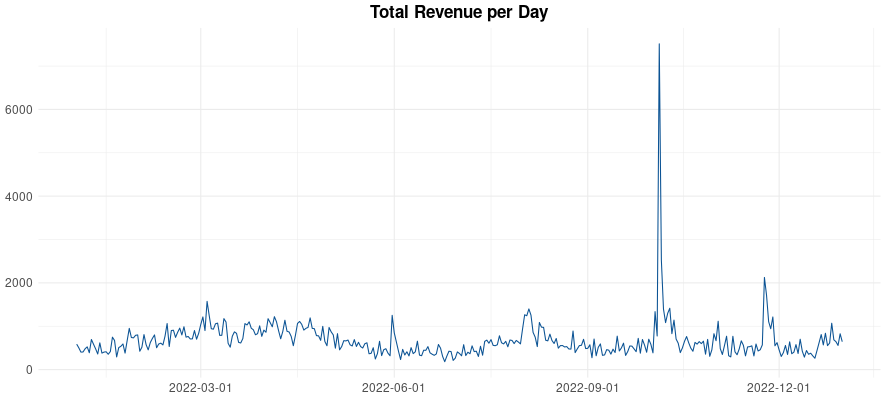
\includegraphics[width=\textwidth]{pictures/2_timeline_graph.png}
    \caption{Συνολικός τζίρος ανά ημέρα για το 2022}
    \label{fig:2}
\end{figure}

Σημαντικό στοιχείο του dashboard είναι η εύρεση των καλύτερων κατηγοριών, εκδοτικών οίκων και αφηγητών. Σε αυτήν την περίπτωση είναι απαραίτητη η σύγκριση ανάμεσα στις διάφορες τιμές μιας κατηγορικής μεταβλητής βάσει κάποιας μετρικής. Οι δύο πιο συνήθεις λύσεις είναι τα ραβδογράμματα και τα διαγράμματα πίτες. Καθώς όμως τα διαγράμματα πίτες έχουν δεχθεί έντονη κριτική για τη δυσκολία στην ξεκάθαρη κατανόησή τους και τη δυσχέρεια της ανθρώπινης αντίληψης να διακρίνει ενστικτωδώς τα πραγματικά μεγέθη, το διάγραμμα που θα χρησιμοποιηθεί είναι το ραβδόγραμμα. Για παράδειγμα, με δεδομένες τις καλύτερες 10 κατηγορίες βιβλίων βάσει του συνολικού κέρδους, ορίζουμε ως αρχική αισθητική στον άξονα y τις κατηγορίες, και στον άξονα x το συνολικό κέρδος. Ο λόγος για τον οποίο έχουμε τις κατηγορίες στον άξονα y και όχι στον άξονα x, είναι διότι, σε περίπτωση που μια κατηγορία έχει μεγάλο όνομα, είναι πιο ευανάγνωστη οριζόντια απ’ότι κάθετα, αξιοποιώντας καλύτερα και το χώρο του διαγράμματος. Ως γεωμετρία, ορίζουμε τις στήλες με τη συνάρτηση geom\_col για τη δημιουργία ράβδων. Όπως και προηγουμένως, οι υπόλοιπες αλλαγές αφορούν την αισθητική του διαγράμματος. Οι τίτλοι και τα μεγέθη των γραμματοσειρών έγιναν με την ίδια λογική, όπως και στο προηγούμενο διάστημα, και η μόνη διαφορά είναι στο χρώμα των ράβδων, όπου χρησιμοποιήθηκε διαβάθμιση χρώματος, προκειμένου να τονίσει τις πιο καλές κατηγορίες (εικόνα 3).

\begin{figure}[h]
    \centering
    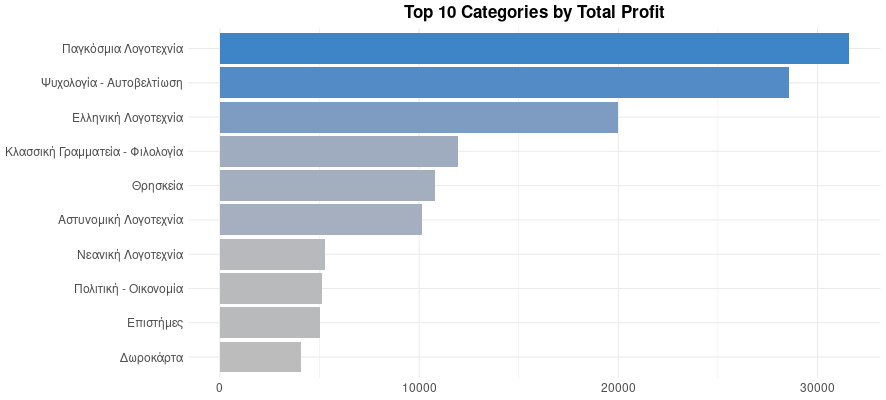
\includegraphics[width=\textwidth]{pictures/3_bar_graph.png}
    \caption{Οι δέκα καλύτερες κατηγορίες βιβλίων με βάση το συνολικό κέρδος}
    \label{fig:3}
\end{figure}

Για τις μετρικές βάσει της χώρας παραγγελίας, οι επιλογές είναι όπως και στην προηγούμενη περίπτωση κάποιο ραβδόγραμμα, αν το επιθυμητό αποτέλεσμα είναι οι καλύτερες σε κάποια μετρική χώρες, ή ένα διάγραμμα χάρτη. Επιλέχθηκε το διάγραμμα χάρτη, καθώς παρέχει μια γενικότερη και πιο ολοκληρωμένη εικόνα. Πέραν των δεδομένων ανά χώρα, απαραίτητα είναι και τα δεδομένα για τη δημιουργία των χαρτών. Η R προσφέρει βιβλιοθήκες οι οποίες περιέχουν δεδομένα χαρτών για διευκόλυνση του χρήστη. Τα δεδομένα αυτά πρέπει να συνδυαστούν με τα δεδομένα του ηλεκτρονικού καταστήματος, προκειμένου να επιτευχθεί το επιθυμητό αποτέλεσμα. Για παράδειγμα, αν θέλουμε να δούμε το μέσο κέρδος, έχοντας ως δεδομένο το σύνολο που έχει συνδέσει τις συντεταγμένες με τα στοιχεία των πωλήσεων ανά χώρα, ορίζεται αρχικά η αισθητική με το γεωγραφικό μήκος στον άξονα x και το γεωγραφικό πλάτος στον άξονα y, μια μεταβλητή ομαδοποίησης (παρέχεται από τα δεδομένα συντεταγμένων) και στο γέμισμα των χωρών το μέσο κέρδος. Έπειτα, η γεωμετρία είναι τα πολύγωνα τα οποία δημιουργούνται βάσει των συντεταγμένων. Ως προς τις συντεταγμένες, για να είναι πιο όμορφο στο ανθρώπινο μάτι, πρέπει να κληθεί μια συνάρτηση με όνομα coord\_quickmap η οποία μετασχηματίζει το χάρτη σε μορφή Mercator. Τα υπόλοιπα στοιχεία αφορούν τα αισθητικά, με παρόμοιες επιλογές όπως στο ραβδόγραμμα προηγουμένως. Μία σημαντική σημείωση, στις χώρες που δεν υπάρχει δραστηριότητα έχει επιλεγεί σκούρο γκρι χρώμα, ενώ για τις υπόλοιπες υπάρχει διαβάθμιση χρώματος από το ανοιχτό γκρι στο μπλε (εικόνα \ref{fig:4}). Προφανώς όλα αυτά τα στοιχεία μπορούν να προσαρμοσθούν.

\begin{figure}[h]
    \centering
    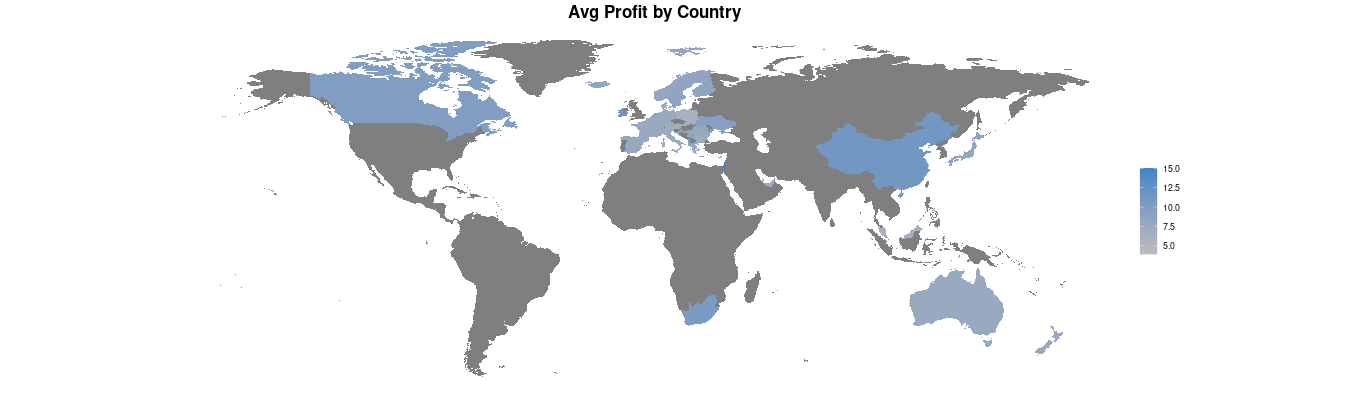
\includegraphics[width=\textwidth]{pictures/4_map_graph.png}
    \caption{Το μέσο κέρδος ανά χώρα}
    \label{fig:4}
\end{figure}

Το τελευταίο είδος γραφήματος που χρειαζόμαστε είναι η απεικόνιση ανά χρονική μονάδα. Το διάγραμμα γραμμής που χρησιμοποιήθηκε προηγουμένως απεικονίζει με πολύ καλό τρόπο την ιστορικότητα, αλλά δεν ταιριάζει σε αυτήν την περίπτωση όπου θέλουμε ο χρόνος να αντιμετωπίζεται όπως μία κατηγορική μεταβλητή. Σε αντίθεση βέβαια με τις μεταβλητές αυτές, είναι σημαντικό να τηρείται και η σειρά του χρόνου για να μην αλλοιωθεί η ανθρώπινη αντίληψη, για παράδειγμα στον μέσο τζίρο ανά ημέρα της εβδομάδας δε θα είχε νόημα να ήταν η Τρίτη πριν από τη Δευτέρα, το Σάββατο δίπλα από την Τετάρτη και ούτω καθεξής. Το πιο αποδοτικό διάγραμμα θα ήταν ένα ραβδόγραμμα ταξινομημένο ανά ημέρα της εβδομάδας (στον άξονα x) όπου θα εμφανίζεται ο μέσος τζίρος (άξονας y), με τις στήλες να αποτελούν τη γεωμετρία του. Τα υπόλοιπα αισθητικά είναι όπως και προηγουμένως, με τη διαφορά ότι όλες οι ράβδοι έχουν το ίδιο χρώμα. (εικόνα \ref{fig:5})

\begin{figure}[h]
    \centering
    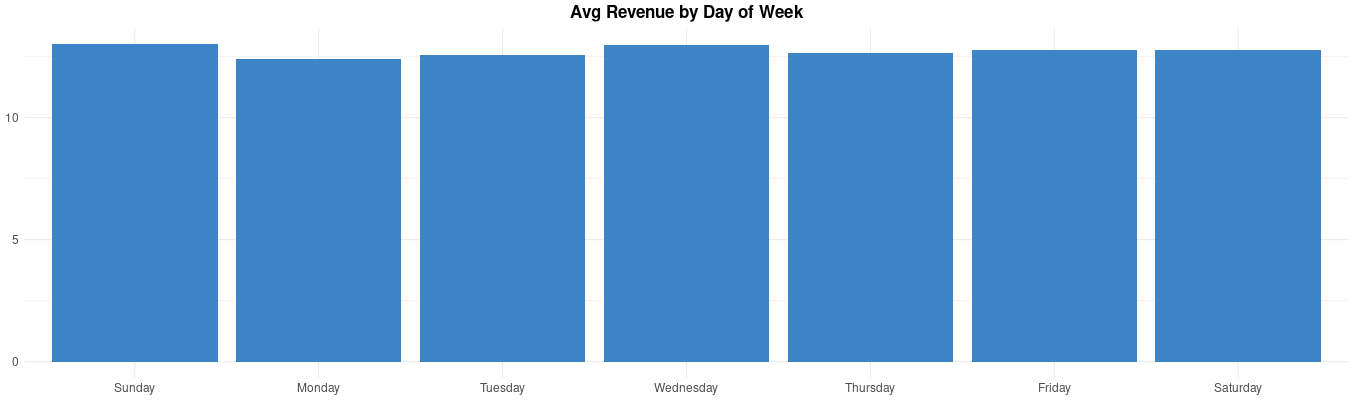
\includegraphics[width=\textwidth]{pictures/5_timebar_graph.png}
    \caption{Μέσος τζίρος ανά ημέρα της εβδομάδας}
    \label{fig:5}
\end{figure}

\subsection{Υλοποίηση του Dashboard}

Έχοντας στη διάθεσή μας τα γραφήματα, πλέον μπορούμε να προχωρήσουμε στην υλοποίηση του dashboard. Αρχικά, θα παρθεί η απόφαση για τη διαρρύθμισή του. Καθώς, θα δίνεται και η δυνατότητα για συσταδοποίηση, θα ήταν σκόπιμο να είναι διακριτές οι λειτουργίες. Επομένως, επιλέχθηκε μια διάταξη τύπου καρτελών, που θα διαχωρίζει την εφαρμογή σε τρεις καρτέλες: το Dashboard, τα δεδομένα και τη συσταδοποίηση. (Εικόνα \ref{fig:6})

\begin{figure}[h]
    \centering
    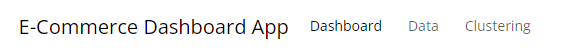
\includegraphics[width=\textwidth]{pictures/6_navbar.png}
    \caption{Διάταξη των καρτελών, με παρούσα καρτέλα το dashboard}
    \label{fig:6}
\end{figure}

\subsubsection{Καρτέλα Dashboard}

Η πρώτη και πιο σημαντική καρτέλα είναι το ίδιο το Dashboard. Σε αυτήν την καρτέλα τοποθετούνται όλα τα γραφήματα που δημιουργήθηκαν στην προηγούμενη ενότητα. Κάθε καρτέλα αναπαρίσταται στο Shiny με τη συνάρτηση tabPanel, οπότε όλο το περιεχόμενο βρίσκεται σε κάθε μία κλήση αυτής της συνάρτησης εντός του αντικειμένου ui. Στη συγκεκριμένη καρτέλα, εκμεταλλευόμαστε τη δομή fluidPage, δηλαδή, η διαρρύθμιση χωρίζεται σε γραμμές οι οποίες με τη σειρά τους αποτελούνται από δώδεκα στήλες. Με αυτόν τον τρόπο είναι πιο εύκολη η διαχείριση της εφαρμογής και η τοποθέτηση των διαφόρων στοιχείων. Κάθε γραμμή αναπαρίσταται από τη συνάρτηση fluidRow, και η διαχείριση των στηλών γίνεται είτε από τη συνάρτηση column\_layouts είτε από τη column\_layout\_wrap. Για ακόμα περισσότερο έλεγχο και προσαρμογή, τα περισσότερα στοιχεία βρίσκονται σε μία συνάρτηση div, η οποία δημιουργεί ένα «container».

Στην πρώτη γραμμή, βρίσκονται τα φίλτρα που αφορούν όλο το dashboard. Αυτό σημαίνει ότι αλλαγή σε ένα από αυτά επηρεάζει όλα τα γραφήματα που ακολουθούν. Συνήθως είναι καλή πρακτική τα φίλτρα να βρίσκονται στην αρχή ενός dashboard από τη στιγμή που το ανθρώπινο μάτι μπορεί να τα βρει πολύ πιο εύκολα. Όσον αφορά τα ίδια τα φίλτρα, κατά βάση έχουν χρησιμοποιηθεί όλες οι κατηγορικές μεταβλητές και η ημερομηνία. Σαφώς, θα μπορούσε να υπάρχει και η δυνατότητα προσαρμοσμένου φίλτρου ή και πιο σύνθετων συνθηκών, αλλά ξεφεύγει από το αντικείμενο της συγκεκριμένης μελέτης. Όπως φαίνεται και στο παρακάτω απόκομμα \ref{snippet:1}, η κύρια συνάρτηση είναι το selectInput, το οποίο δέχεται σαν παραμέτρους το id του φίλτρου που θα χρησιμοποιηθεί στις συναρτήσεις του server, το όνομα-ετικέτα που θα φαίνεται στο χρήστη, οι διαθέσιμες επιλογές (όλες οι δυνατές τιμές της μεταβλητής και επιλογή όλα) και η αρχική επιλογή. Τα υπόλοιπα στοιχεία του div είναι στυλιστικά. Το συνολικό αποτέλεσμα των φίλτρων φαίνεται στην εικόνα \ref{fig:7}.

\begin{figure}[h]
    \centering
    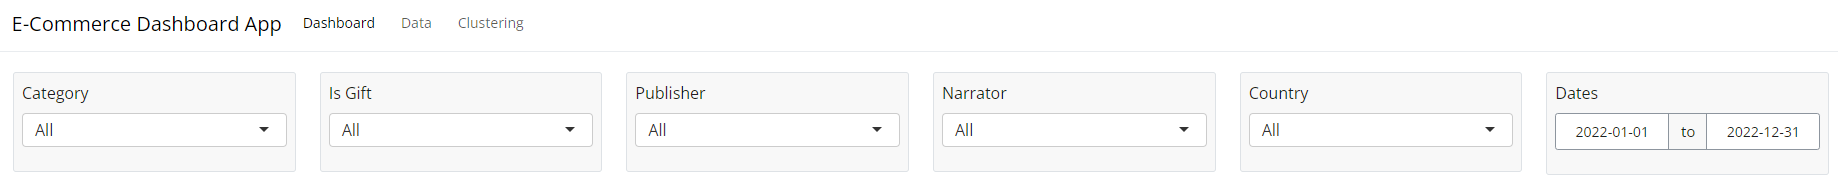
\includegraphics[width=\textwidth]{pictures/7_filters.png}
    \caption{Φίλτρα σελίδας στο πάνω μέρος του dashboard}
    \label{fig:7}
\end{figure}

\begin{lstlisting}[language=R, caption=Container φίλτρων, label={snippet:1}]  
    div(
        class = 'border rounded-2 p-2',
        style = 'background-color: #f8f8f8',
        selectInput('category', 
         'Category', 
         choices = c('All', unique(sales_data$category)), 
         selected = 'All')
    ),
\end{lstlisting}

Κάθε φορά που εφαρμόζεται ένα φίλτρο, ο server εκτελεί μία συνάρτηση η οποία φιλτράρει τα δεδομένα, και τα διαθέτει μετέπειτα στις γραφιστικές συναρτήσεις για χρήση. (απόκομμα \ref{snippet:2}) Χρησιμοποιώντας τη συνάρτηση filter της βιβλιοθήκης dplyr, κρατάμε για κάθε μία κατηγορική μεταβλητή την τιμή του φίλτρου.

\begin{lstlisting}[language=R, caption=Φιλτράρισμα δεδομένων, label={snippet:2}]
    filtered <- reactive(
    {
      date1 <- input$dates[1]
      date2 <- input$dates[2]
      df <- sales_data %>%
        dplyr::filter(order_date >= date1 & order_date <= date2 &
             (input$category == 'All' |
               input$category == category) &
             (input$is_gift == 'All' |
               input$is_gift == is_gift) &
             (input$publisher == 'All' |
               input$publisher == publisher) &
             (input$narrator == 'All' |
               input$narrator == narrator) &
             (input$country == 'All' |
               input$country == country))
      return(df)
    }
  )
\end{lstlisting}

Η δεύτερη γραμμή περιέχει τις οπτικοποιήσεις καρτών. (εικόνα \ref{fig:8}) Για καθεμία από τις μετρικές που εξετάζονται δημιουργείται μία κάρτα με τη συνάρτηση του αποκόμματος \ref{snippet:3}. Η συνάρτηση textOutput δέχεται τη μετρική και σε μιά άλλη συνάρτηση στο server επιστρέφει το άθροισμα για τη μετρική αυτή ως κείμενο για να χρησιμοποιηθεί στην κάρτα. Αυτή η συνάρτηση διευκολύνει τη δημιουργία καρτών εντός του ui, μιας και δε χρειάζεται να γράφεται ο ίδιος κώδικας πολλές φορές. Η γραμμή χρησιμοποιεί το layout\_column\_wrap αξιοποιώντας τέσσερις στήλες, ίδιου μεγέθους όπως φαίνεται στο απόκομμα \ref{snippet:4}.

\begin{figure}[h]
    \centering
    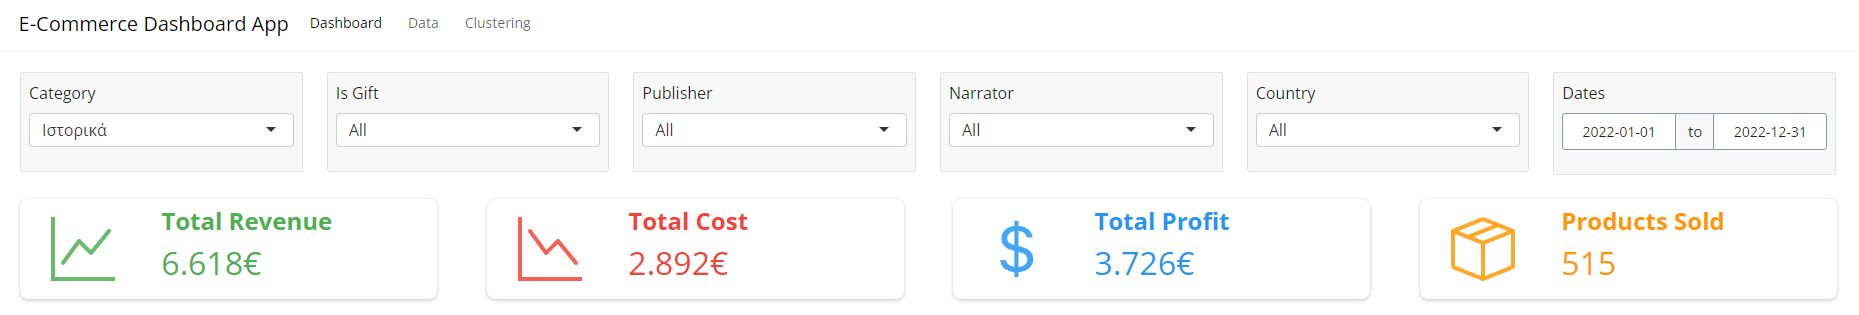
\includegraphics[width=\textwidth]{pictures/8_card_visuals.png}
    \caption{Οπτικοποιήσεις κάρτας στο dashboard κάτω από τα φίλτρα}
    \label{fig:8}
\end{figure}

\begin{lstlisting}[language=R, caption=Φιλτράρισμα δεδομένων, label={snippet:3}]
card_visual <- function(card, title, bgcolor, icon, fgcolor) {
  return(value_box(
    title = p(title, style = 'font-weight: bold; font-size: 24px'), 
    value = textOutput(card),
    theme = value_box_theme(bg = bgcolor, fg = fgcolor),
    showcase = bsicons::bs_icon(icon), showcase_layout = "left center",
    full_screen = FALSE, fill = TRUE, height = NULL
  ))
}
\end{lstlisting}

\begin{lstlisting}[language=R, caption=Φιλτράρισμα δεδομένων, label={snippet:4}]
fluidRow(
    layout_column_wrap(
        width = 1/4,
        height = '100px',
        fixed_width = T,
        gap = 50,
        card_visual('revenue', 'Total Revenue', 'grey90', 'graph-up', '#4CAF50'),
        card_visual('cost', 'Total Cost', "grey90", 'graph-down', '#F44336'),
        card_visual('profit', 'Total Profit', "grey90", 'currency-dollar', '#2196F3'),
        card_visual('quantity_sold', 'Products Sold', "grey90", 'box-seam', '#FF9800')
    )
),
\end{lstlisting}

Στο σημείο αυτό να σημειωθεί πώς δε θα περιλαμβάνονται τα αποκόμματα του κώδικα εντός του κειμένου για τα επόμενα γραφήματα, καθώς αυξάνεται ο αριθμός των γραμμών, και σε γενικές γραμμές ακολουθείται η ίδια διαδικασία. Αρχικά καλούνται τα φιλτραρισμένα δεδομένα, από τα οποία κρατώνται μόνο οι στήλες οι οποίες έχουν επιλεχθεί για κάθε διάγραμμα. Έπειτα γίνεται μια μετονομασία των στηλών με πιο γενικευμένα ονόματα, προκειμένου να εξασφαλισθεί η επεκτασιμότητα της εφαρμογής, ομαδοποιούνται τα δεδομένα, συναθροίζονται και τέλος δημιουργείται και επιστρέφεται το γράφημα. Ο κώδικας, όπως είχε αναφερθεί και προηγουμένως βρίσκεται διαθέσιμος τόσο στο \href{https://github.com/kostas-rigan/r-shiny-dashboard-app}{GitHub}, όσο και στο παράρτημα.

Η επόμενη γραμμή περιέχει δύο είδη γραφημάτων, το χρονοδιάγραμμα και το ραβδόγραμμα. (εικόνα \ref{fig:9}) Συνήθως άλλα dashboard περιέχουν πολλά ίδια διαγράμματα με ελάχιστες αλλαγές μεταξύ αυτών, συνήθως στο κομμάτι των μετρικών. Όμως το Shiny παρέχει πολλές δυνατότητες προσαρμογής, δίνοντας την επιλογή να αλλάζουμε το γράφημα, με ελάχιστα κλικ. Στα δύο διαγράμματα, προτιμήθηκε η χρήση του γραναζιού για τις ρυθμίσεις του κάθε γραφήματος όπως φαίνεται στην εικόνα \ref{fig:10}, καθώς είναι κάτι που έχει συνηθίσει ο χρήστης σε άλλες εφαρμογές με βάση τη δεύτερη ευρετική του Nielsen. Για κάθε γράφημα στο εξής, οι κοινές ρυθμίσεις είναι η μετρική και η συναθροιστική συνάρτηση. Εφόσον σκοπός είναι να βλέπει ο δέκτης του dashboard τον τζίρο, το κόστος, το κέρδος κτλ υπό διαφορετικό πρίσμα, για παράδειγμα μέσο ή συνολικό, κάθε μία ρύθμιση έχει αυτές τις παραμέτρους. Οι διαθέσιμες μετρικές είναι ο τζίρος, το κόστος και το κέρδος, ενώ οι συναθροιστικές συναρτήσεις το άθροισμα, η μέση τιμή, η διάμεσος και η συχνότητα. Φυσικά, θα μπορούσαν να προστεθούν παραπάνω μετρικές και συναρτήσεις συνάθροισης, αλλά για τους σκοπούς της συγκεκριμένης μελέτης αρκούν τα παραπάνω. Για κάθε γράφημα υπάρχουν επίσης και διαφορετικοί παράμετροι. Στο χρονοδιάγραμμα δίνεται η δυνατότητα μέσω φυσικής γλώσσας να ορίζει τα χρονικά διαστήματα στα οποία θα υπάρχει tick. Αυτό είναι εφικτό χάρη στη δυνατότητα του ggplot για διαγράμματα με μεταβλητή άξονα τον χρόνο να ορίζει τα breaks. Για το ραβδόγραμμα, ο χρήστης μπορεί να επιλέξει ανάμεσα στις διαθέσιμες κατηγορικές μεταβλητές, όπως επίσης και πόσα αντικείμενα θα φαίνονται (από 1-10).

\begin{figure}[h]
    \centering
    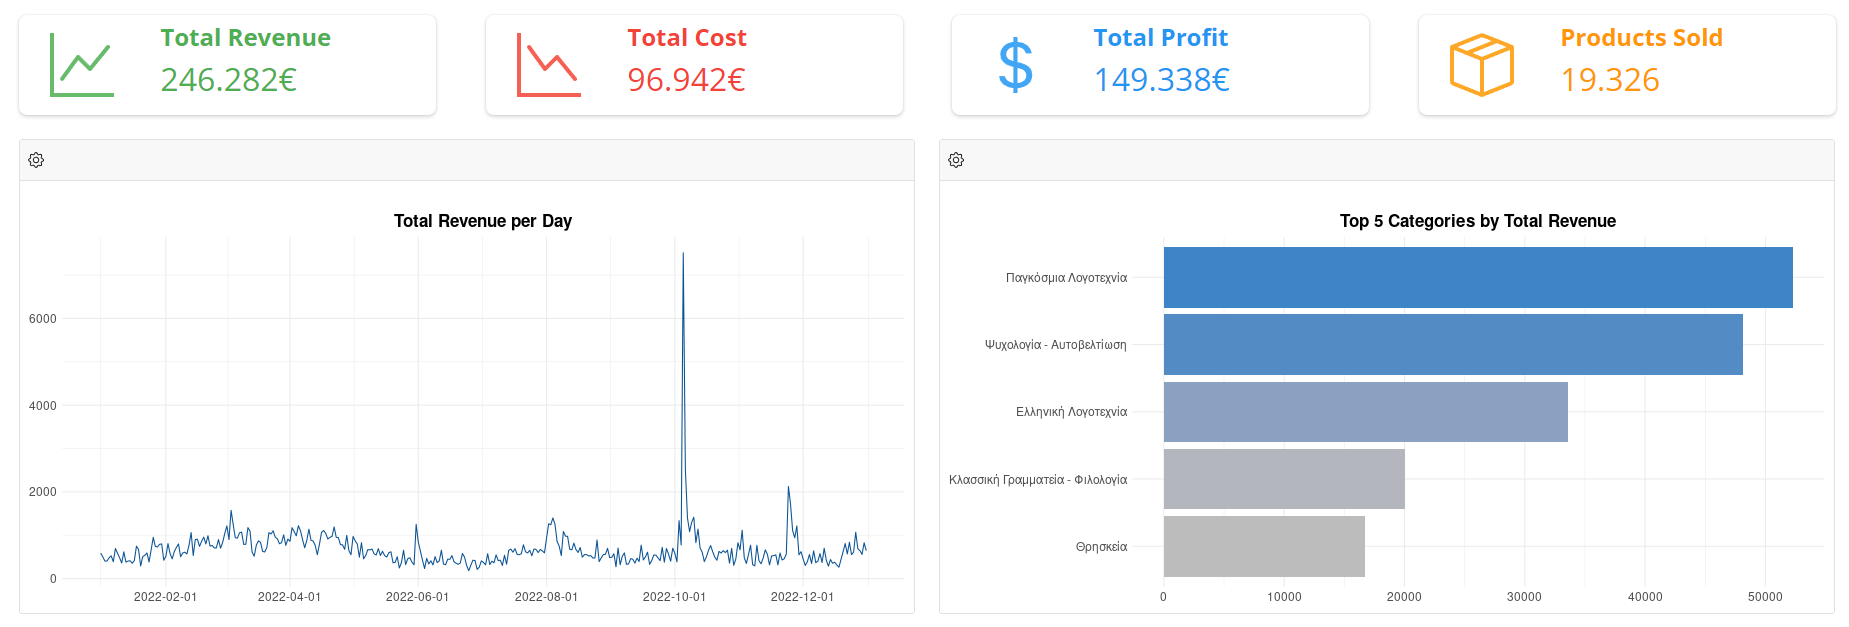
\includegraphics[width=\textwidth]{pictures/9_timeline_bar_visuals.png}
    \caption{Οπτικοποιήσεις χρονοδιαγράμματος και ραβδογράμματος}
    \label{fig:9}
\end{figure}

\begin{figure}[h]
    \centering
    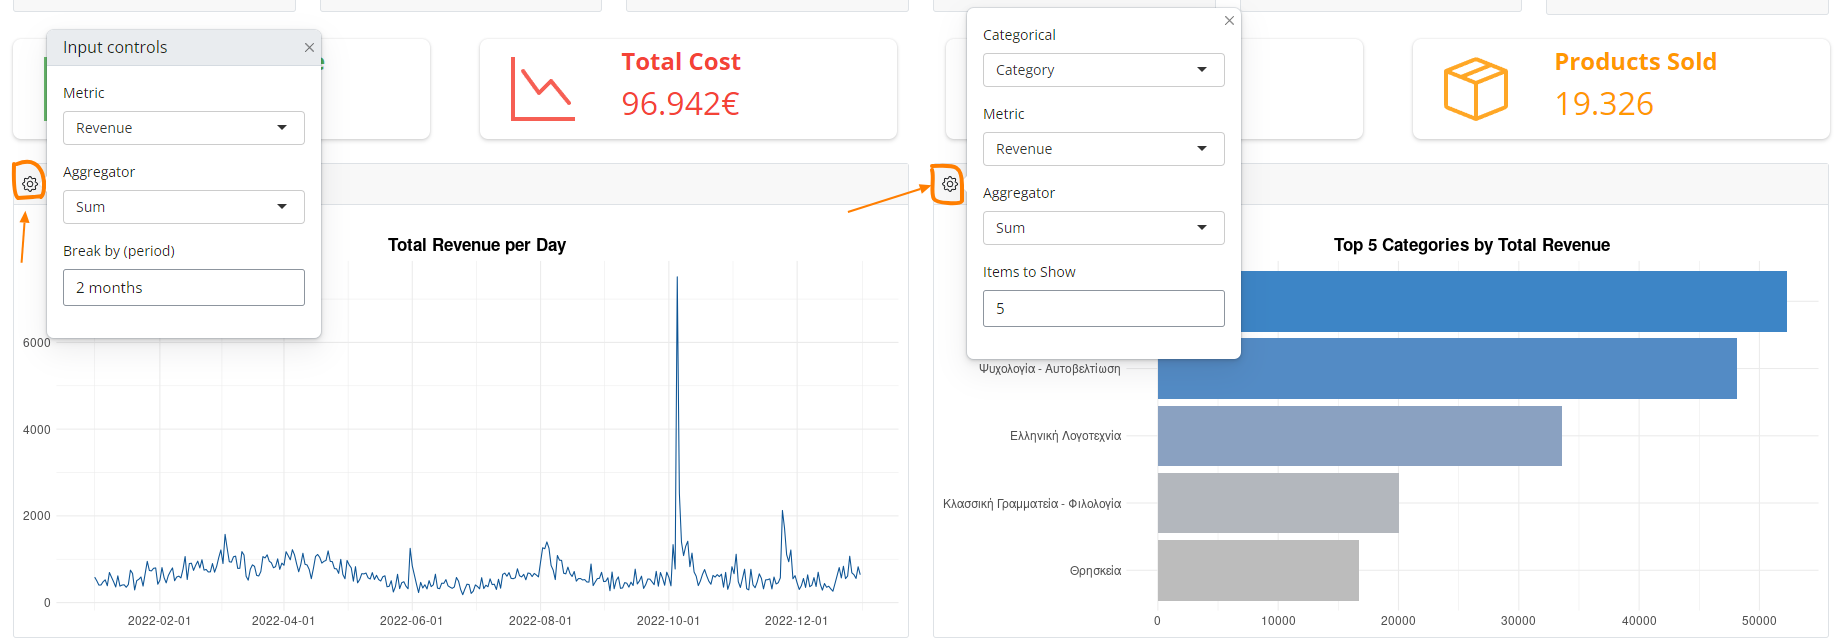
\includegraphics[width=\textwidth]{pictures/10_timeline_bar_visuals_open_filters.png}
    \caption{Ρυθμίσεις χρονοδιαγράμματος και ραβδογράμματος}
    \label{fig:10}
\end{figure}

Η επόμενη γραμμή περιλαμβάνει το χάρτη. Σε αντίθεση με τα προηγούμενα δύο γραφήματα, οι ρυθμίσεις βρίσκονται στα αριστερά, διαφορετικά θα υπήρχε αναξιοποίητος χώρος. Η νέα ρύθμιση που υπάρχει είναι ένα checkbox το οποίο δεν συμπεριλαμβάνει την Ελλάδα στην ανάλυση. Είναι πολύ προσαρμοσμένο στη συγκεκριμένη περίπτωση μιας και η Ελλάδα αποτελεί την κύρια χώρα εσόδων και κερδών, επομένως κάτι τέτοιο μπορεί να διευκολύνει τα στελέχη να πάρουν πιο στρατηγικές αποφάσεις. Στο server πρακτικά, με τον ίδιο τρόπο που είδαμε και παραπάνω, η αντίστοιχη συνάρτηση φιλτράρει εκτός την Ελλάδα εφόσον είναι ενεργό. Στην εικόνα \ref{fig:11}, είναι ο συνολικός τζίρος ανά χώρα με εξαίρεση την Ελλάδα.

\begin{figure}[h]
    \centering
    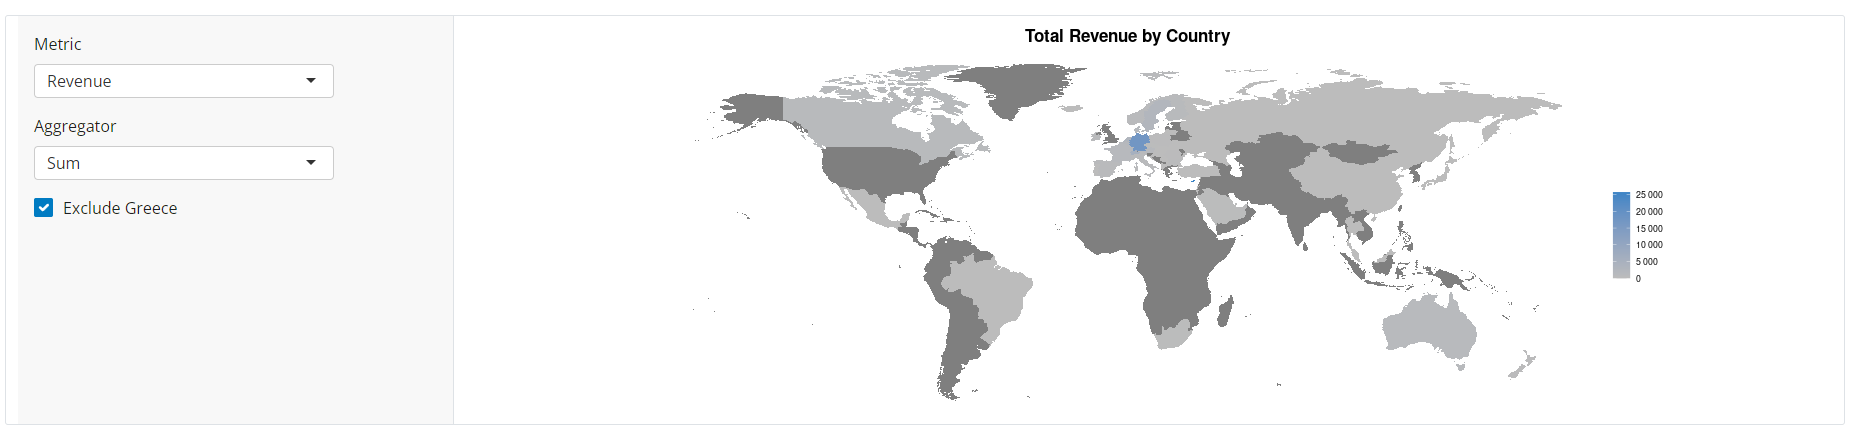
\includegraphics[width=\textwidth]{pictures/11_map_visual.png}
    \caption{Οπτικοποίηση χάρτη}
    \label{fig:11}
\end{figure}

Στην τελευταία γραμμή βρίσκεται το διάγραμμα ανά χρονικό διάστημα. Η διάταξη ίδια με το διάγραμμα χάρτη, όμως η ξεχωριστή ρύθμιση είναι η επιλογή του διαστήματος. (εικόνα \ref{fig:12}) Ο χρήστης θα μπορεί να επιλέξει ανάμεσα σε μέρα της εβδομάδας, το μήνα και την ώρα της ημέρας.

\begin{figure}[h]
    \centering
    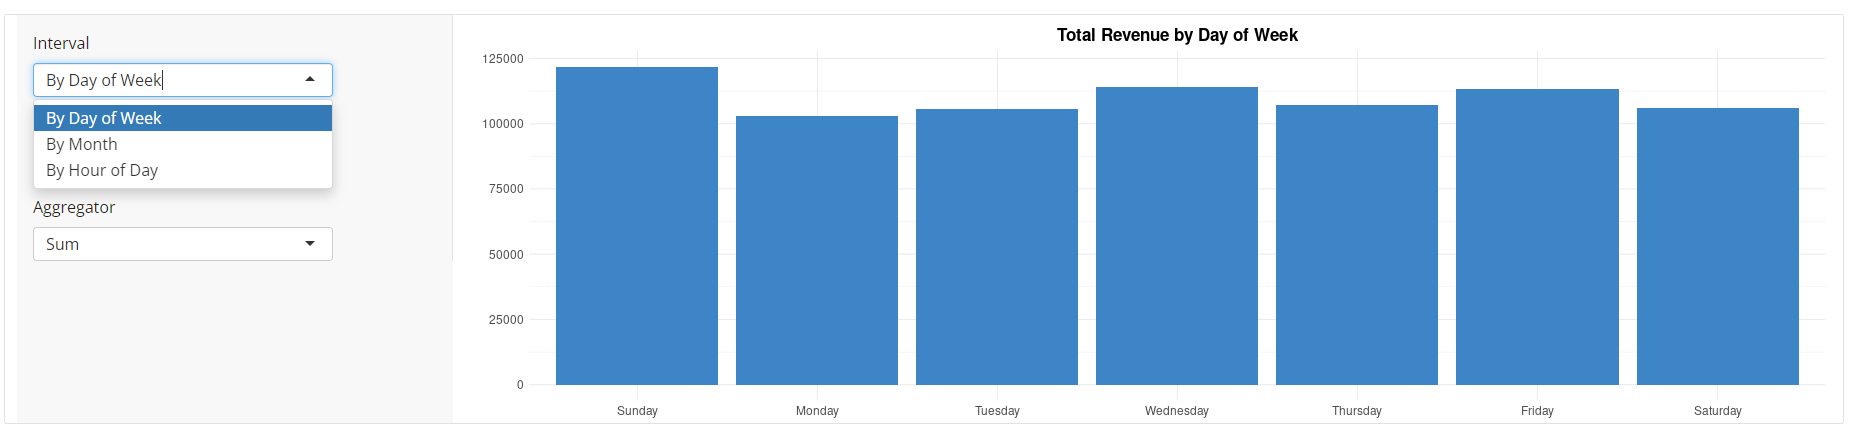
\includegraphics[width=\textwidth]{pictures/12_timebar_visual.png}
    \caption{Οπτικοποίηση ραβδογράμματος ανά χρονική περίοδο}
    \label{fig:12}
\end{figure}

\subsubsection{Καρτέλες Data και Clustering}

Σε επόμενο tabPanel βρίσκεται ένας πίνακας ο οποίος περιέχει τα δεδομένα σε μορφή πίνακα. Δεν εξυπηρετεί σε κάτι παραπάνω πέρα από μία γρήγορη ματιά και γνωριμία με τα δεδομένα με τα οποία δουλεύει ο χρήστης. Ακολουθούν το αντίστοιχο απόκομμα \ref{snippet:5} και η αντίστοιχη εικόνα (εικόνα \ref{fig:13}). 

\begin{lstlisting}[language=R, caption=Κώδικας για τον πίνακα δεδομένων, label={snippet:5}]
tabPanel('Data',       
    DT::dataTableOutput('dataTable')
),
\end{lstlisting}

\begin{figure}[h]
    \centering
    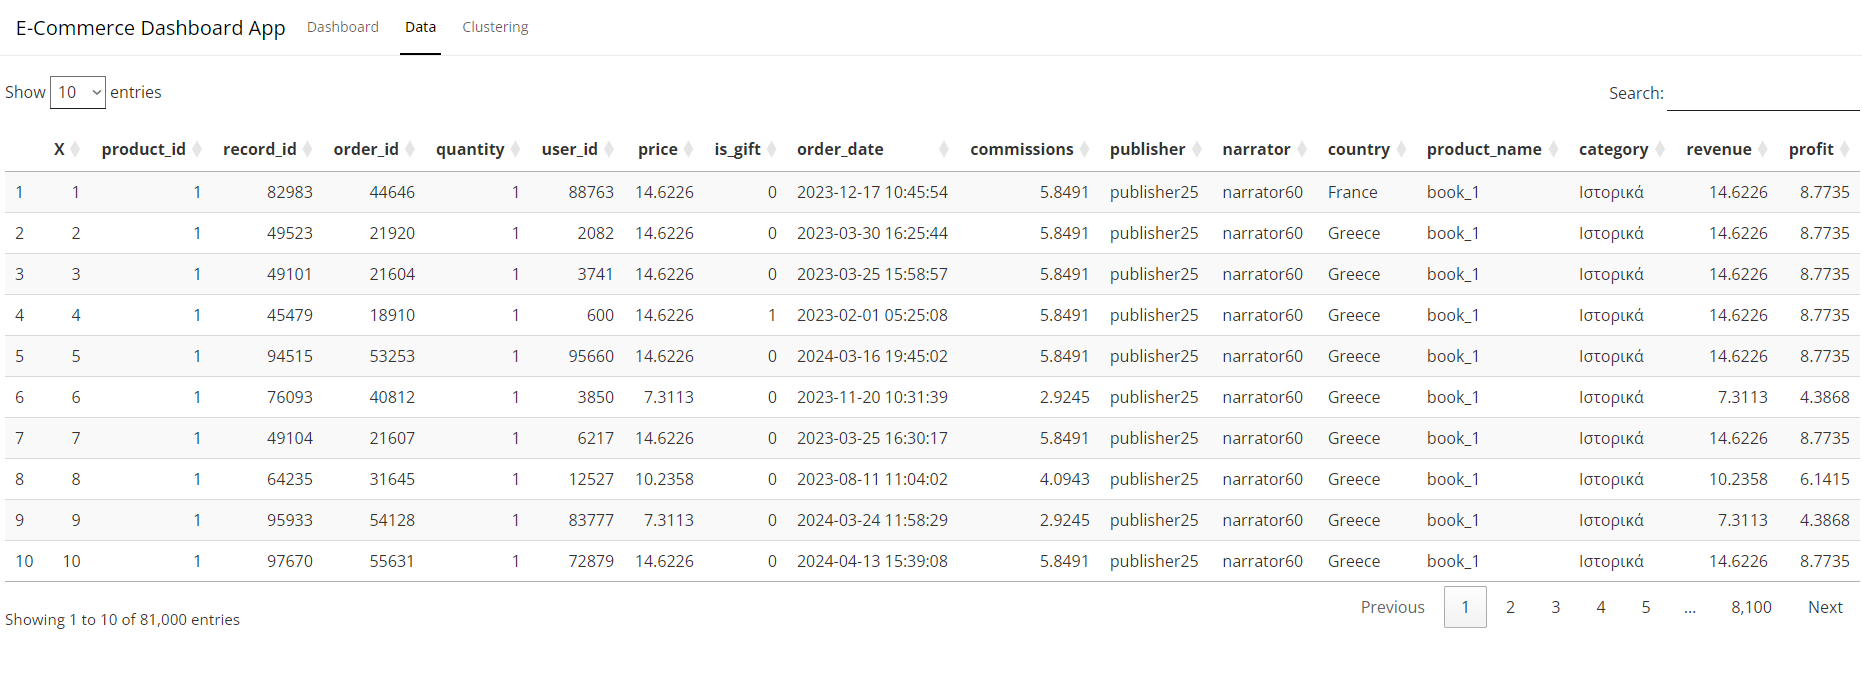
\includegraphics[width=\textwidth]{pictures/13_data_table.png}
    \caption{Πίνακας δεδομένων}
    \label{fig:13}
\end{figure}

Μια λειτουργία η οποία ακόμα δεν έχει συζητηθεί στο στάδιο της υλοποίησης είναι η συσταδοποίηση. Αν και ακόμα δεν είναι σε επίπεδο παραγωγής, υπάρχει η δυνατότητα για κάποιες δοκιμές και αποτελέσματα διαθέσιμα προς λήψη. Μέσα στο tabPanel χρησιμοποιείται μία διαφορετική δομή το sidebarLayout, δηλαδή μία διάταξη η οποία στο αριστερό της άκρο περιλαμβάνει ένα μενού και στο δεξί το κύριο πάνελ. Ο κώδικας για το sidebar παρουσιάζεται στο απόκομμα \ref{snippet:6}.

\begin{lstlisting}[language=R, caption=Κώδικας του sidebar, label={snippet:6}]
sidebarPanel(
    class = 'h-100',
    style = 'background-color: #f8f8f8',
    h1('K-Means Parameters'),
    p(tags$i('Note: In this version all tests are conducted from k = 1 to 10')),
    hr(),
    h3('General Options'),
    p(tags$i('These options are applied to both testing and running k-means')),
    selectInput('segmentation_var', label = 'Segment:', choices = c('Customers' = 'user_id', 'Orders' = 'order_id')),
    selectInput('clustering_var', label = "By Variable:", choices = c('Category' = 'category', 'Narrator' = 'narrator')),
    hr(),
    h3('Testing Options'),
    p(tags$i('These options apply only in testing k-means with Elbow and Silhouette Method')),
    sliderInput('sample_size', 'Sample Size (%):', value = 0.5, min = 0, max = 1, step = 0.01),
    div(
      class="d-flex justify-content-center",
      actionButton('run_tests', 'Run Test!', class = 'custom-button')
    ),
    hr(),
    h3('k Options'),
    p(tags$i('These options only affect non-testing execution of k-means')),
    numericInput('k', 'k', value = 2, min = 2, max = 10, step = 1),
    div(
      class="d-flex justify-content-center",
      actionButton('run_kmeans', 'Run K-Means!', class = 'custom-button')
    )
    
),
\end{lstlisting}

Απόσπασμα του αποτελέσματος στην εφαρμογή ίσως βοηθήσει στην κατανόηση του κώδικα. (εικόνα \ref{fig:14}) Στο συγκεκριμένο μενού ρυθμίσεων ο χρήστης μπορεί να μεταβάλλει διάφορες παραμέτρους που αφορούν α) όλο το clustering συνολικά (general options), β) τις δοκιμές (testing options) και γ) την εκτέλεση του clustering (k options). Στις γενικές ρυθμίσεις, ο χρήστης μπορεί να ορίσει την οντότητα στην οποία θα κάνει τη συσταδοποίηση (πελάτες ή καλάθια) και πάνω σε ποια μεταβλητή θα γίνει. Έχουν επιλεχθεί μόνο δύο κατηγορικές μεταβλητές για χάριν παραδείγματος, και κάλλιστα θα μπορούσαν να επιλεχθούν και αριθμητικές μεταβλητές, που ενδεχομένως να ήταν πιο εύκολες στη χρήση. Στις ρυθμίσεις δοκιμών ο χρήστης μπορεί να επιλέξει το μέγεθος (\%) του δείγματος στο οποίο θα τρέξει τη συσταδοποίηση, και τέλος στης ρυθμίσεις εκτέλεσης μπορεί να επιλέξει το k (από 1-10). 

\begin{figure}[h]
    \centering
    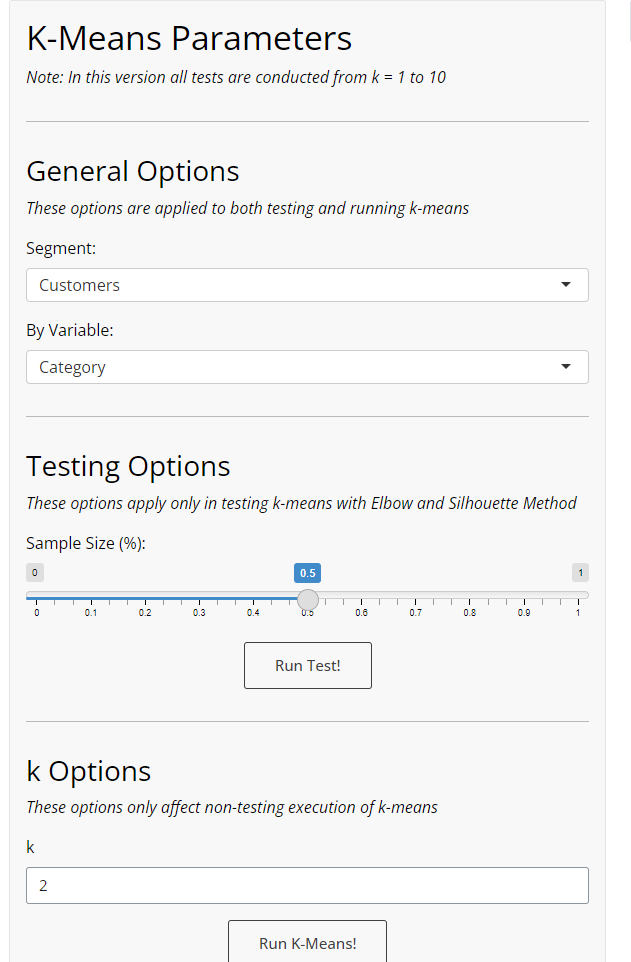
\includegraphics[height=10cm]{pictures/14_sidebar.png}
    \caption{Sidebar στο μενού συσταδοποίησης}
    \label{fig:14}
\end{figure}

Τα δύο κουμπιά έχουν άμεση επίδραση στο κύριο πάνελ. Το κουμπί δοκιμών παράγει τα διαγράμματα αγκώνα (εικόνα \ref{fig:15}, απόκομμα \ref{snippet:7}) και σιλουέτας (εικόνα \ref{fig:16}, απόκομμα \ref{snippet:8}). Για το διάγραμμα αγκώνα, ο server εκτελεί τον αλγόριθμο 10 φορές για k από 1-10 και αποθηκεύει σε έναν πίνακα το άθροισμα των σφαλμάτων τετραγώνου, κι έπειτα με το ggplot δημιουργείται ένα διάγραμμα με γεωμετρία τόσο τις γραμμές όσο και τα σημεία. Η σιλουέτα έχει μία παράμετρο k, προκειμένου να δημιουργεί το αντίστοιχο γράφημα. Επειδή υπολογιστικά απαιτεί πόρους, ήταν απαραίτητη εισαγωγή ποσοστού δείγματος.

\newpage

\begin{figure}[h]
    \centering
    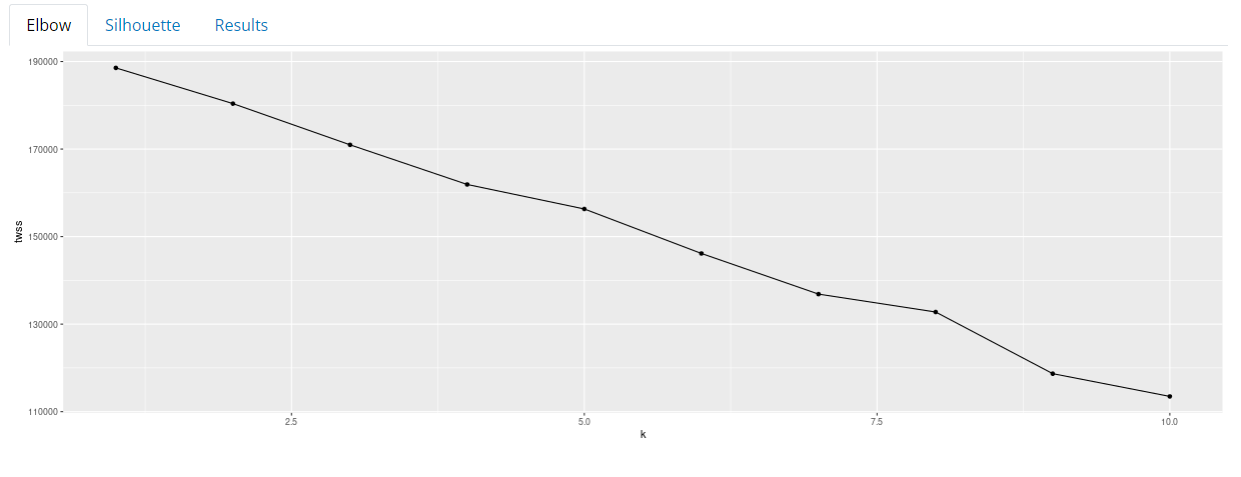
\includegraphics[width=\textwidth]{pictures/15_elbow_method.png}
    \caption{Μέθοδος του αγκώνα}
    \label{fig:15}
\end{figure}

\begin{lstlisting}[language=R, caption=Κώδικας για τη μέθοδο του αγκώνα, label={snippet:7}]
output$elbow <- renderPlot(
    {
      results <- cluster_tests()
      ggplot(results, aes(x = k, y = twss)) + geom_line() + geom_point()
    }
  )
\end{lstlisting}

\begin{figure}[h]
    \centering
    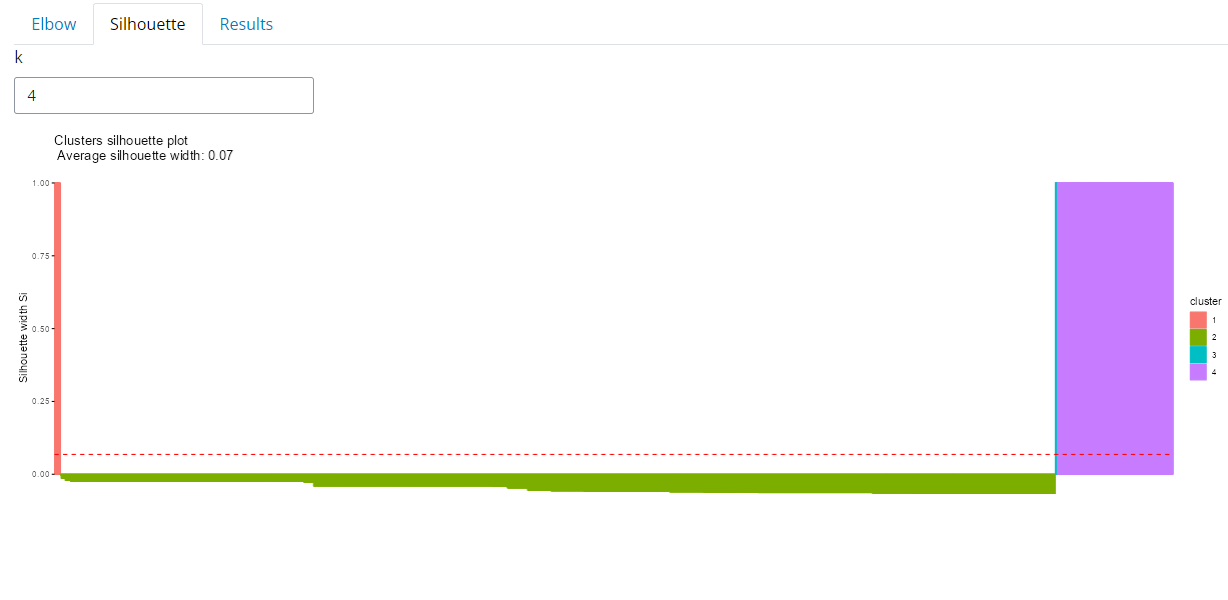
\includegraphics[width=\textwidth]{pictures/16_silhouette_method.png}
    \caption{Μέθοδος της σιλουέτας}
    \label{fig:16}
\end{figure}

\newpage

\begin{lstlisting}[language=R, caption=Κώδικας για τη μέθοδο της σιλουέτας, label={snippet:8}]
output$silhouette <- renderPlot(
    {
      req(input$run_tests)

      sample <- cluster_test_data()
      results <- kmeans(sample[, -1], input$k_sil)
      sil <- silhouette(results$cluster, dist(sample[, -1]))
      fviz_silhouette(sil)
    }
  )
\end{lstlisting}

Το κουμπί εκτέλεσης, δέχεται τον αριθμό k και εκτελεί πλέον με όλα τα δεδομένα τη συσταδοποίηση. Το αποτέλεσμα (απόκομμα \ref{snippet:9}) είναι ένας πίνακας που εμφανίζει τα δεδομένα μαζί με μία καινούρια στήλη, τη συστάδα στην οποία ανήκει. Από εκεί και έπειτα ο χρήστης μπορεί να αποθηκεύσει τα δεδομένα σε ένα αρχείο excel ή csv τοπικά στον υπολογιστή του. (εικόνα \ref{fig:17})

\begin{figure}[h]
    \centering
    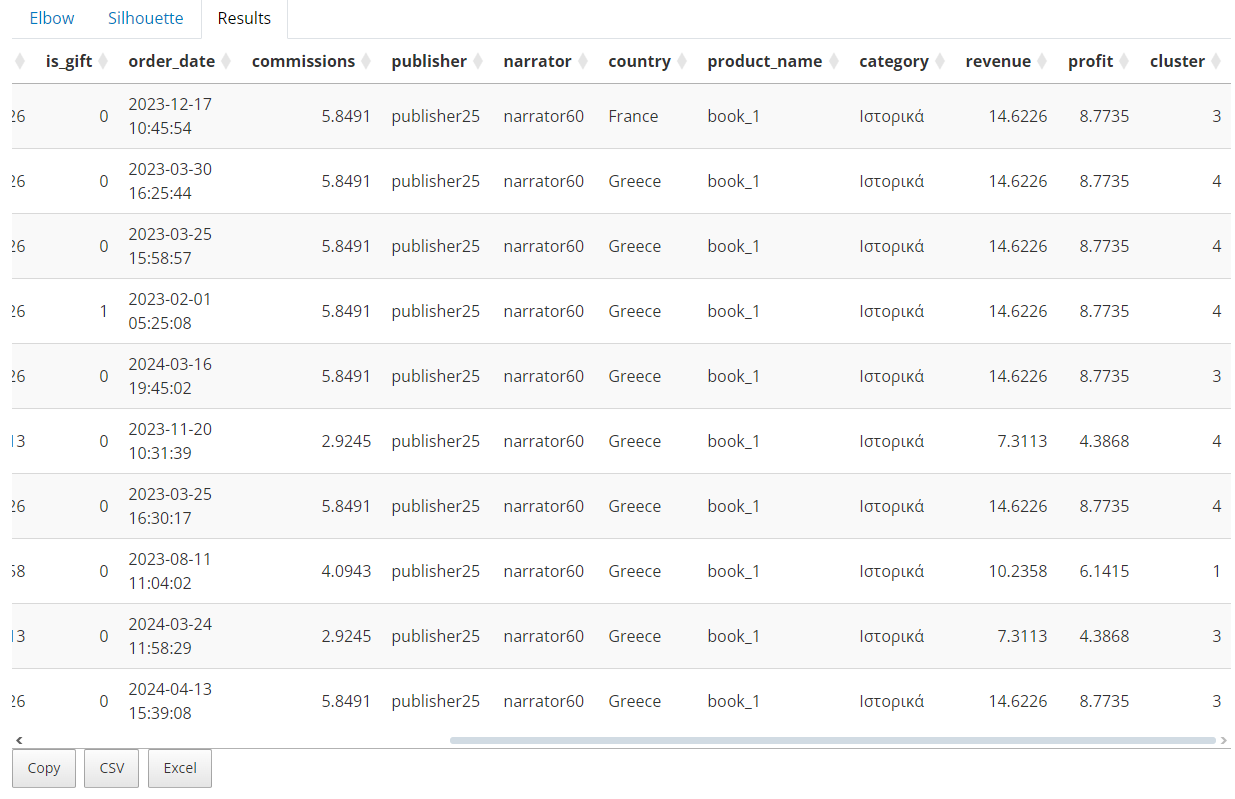
\includegraphics[width=\textwidth]{pictures/17_clustering_results.png}
    \caption{Αποτελέσματα συσταδοποίησης με k=4}
    \label{fig:17}
\end{figure}

\newpage

\begin{lstlisting}[language=R, caption=Κώδικας της συσταδοποίησης, label={snippet:9}]
output$clustering <- renderDataTable(
    {
      req(input$run_kmeans)
      df <- cluster_run_data()
      results <- kmeans(df, centers = input$k)
      df_clu <- as_tibble(data.frame(id = df$seg, cluster = results$cluster))

      temp <- merge(sales_data, df_clu, by.x = input$segmentation_var, by.y = 'id', all.x=T) %>%
        arrange(X) %>%
        filter(duplicated(X) == FALSE)

      DT::datatable(temp,
                    extensions = 'Buttons',
                    options = list(scrollX = TRUE,
                                   paging = TRUE,
                                   searching = TRUE,
                                   fixedColumns = TRUE,
                                   autoWidth = TRUE,
                                   ordering = TRUE,
                                   dom = 'tB',
                                   buttons = c('copy', 'csv', 'excel')))
    }
  )
\end{lstlisting}

\newpage

\section{Αποτελέσματα}

\subsection{Συζήτηση και Περιορισμοί Μελέτης}

Η συγκεκριμένη μελέτη επικεντρώθηκε στη δημιουργία ενός επιχειρησιακού dashboard για δεδομένα ηλεκτρονικού καταστήματος με το R Shiny. Από την ανάλυση φάνηκε πως οι δυνατότητες για προσαρμογή του Shiny ήταν πολλές. Για το ίδιο διάγραμμα, ήταν πολύ απλό να αλλάξει ο χρήστης κάποιες παραμέτρους και να δει αυτό που επιθυμεί από τα δεδομένα. Ο κώδικας για τη δημιουργία του διαγράμματος έχει γραφτεί μία φορά. Η δυσκολία σε αυτήν την περίπτωση έγκειται στη σωστή παραμετροποίηση εντός του κώδικα.

Όσον αφορά τη διεπαφή χρήστη, επίσης το Shiny προσφέρει εσωτερικά πολλές λειτουργίες για τη δημιουργία ενός φιλικού, προς το χρήστη, περιβάλλοντος. Όμως για ακόμη πιο προχωρημένες διεπαφές και για μεγαλύτερο έλεγχο επί αυτών, η HTML και το CSS μπορούν να συνεισφέρουν σημαντικά. Για κάποιον ο οποίος δεν έχει ασχοληθεί με την ανάπτυξη εφαρμογών, και θέλει πιο σύνθετη λειτουργικότητα και διεπαφή χρήστη, θα χρειαστεί σίγουρα εντριβή με τις γλώσσες αυτές.

Το Shiny υποστηρίζει, πέραν του ggplot και άλλες βιβλιοθήκες οπτικοποίησης, όπως είναι το εσωτερικό της πακέτο. Όμως το ggplot και η γραμματική των γραφημάτων, ως φιλοσοφία, διευκολύνουν την ανάπτυξη των γραφημάτων. Για παράδειγμα, στο χρονοδιάγραμμα ο χρήστης έχει τη δυνατότητα να ορίσει τα χρονικά διαστήματα εμφάνισης των ticks. Καθώς κάτι τέτοιο είναι ενσωματωμένο στο ggplot,, η υλοποίηση μιας τέτοιας λειτουργίας δεν έιναι δύσκολη. Όμως, και αυτή η βιβλιοθήκη χρειάζεται χρόνο για εξάσκηση και την πληρέστερη κατανόησή της.

Κάποιοι από τους βασικούς περιορισμούς ήταν σε μεγάλο βαθμό ο χρόνος. Πέραν της εκμάθησης του Shiny και την ανάπτυξη της εφαρμογής, απαραίτητη ήταν και η εκμάθηση της γλώσσας R και των βιβλιοθηκών της όπως dplyr και ggplot2. Τόσο η γλώσσα όσο και οι βιβλιοθήκες απαιτούσαν ώρες μελέτης για να καλυφθούν με τον καλύτερο δυνατό τρόπο οι ανάγκες του dashboard σε έναν ικανοποιητικό βαθμό.

Λειτουργικά, δεν ήταν εφικτό να υλοποιηθεί η δυνατότητα ανάρτησης αρχείου και να είναι σε σύντομο χρονικό διάστημα ολοκληρωμένη. Η συγκεκριμένη περίπτωση θα απαιτούσε ενδεχομένως κάποια γεννήτρια γραφημάτων, δυναμική επιλογή στηλών στα φίλτρα, όπως και ορισμός των μετρικών στην καρτέλα Data. Επίσης δεν προστέθηκαν όλες οι συναθροιστικές συναρτήσεις που θα μπορούσαν, κυρίως γιατί δε θα προσέφεραν κάτι ουσιαστικό στη συγκεκριμένη περίπτωση. Για παράδειγμα, η ελάχιστη και η μέγιστη τιμή σαν συναρτήσεις θα είχαν νόημα να βρίσκονται στο dashboard. Η συσταδοποίηση επίσης επιδέχεται πολλές βελτιώσεις τόσο λειτουργικά όσο και αισθητικά. Σε μια ολοκληρωμένη εφαρμογή, θα ήταν πολύ σημαντικό να υπάρχει η δυνατότητα προσθήκης στήλης στο σύνολο δεδομένων με κάποια εξειδεικευμένη γλώσσα όπως το DAX της Microsoft ή κάποια διεπαφή. Αυτές οι στήλες, μπορούν στη συνέχεια χρησιμοποιούνται σε όλο το υπόλοιπο dashboard, για παράδειγμα είτε σαν φίλτρο είτε στο ραβδόγραμμα. Τα διαγράμματα αγκώνα και σιλουέτας επίσης θα μπορούσαν να έχουν καλύτερη εμφάνιση, όμως λόγω του γεγονότος ότι είναι πειραματικές, δε δόθηκε περισσότερη σημασία.

\subsection{Εκτάσεις για Μελλοντική Έρευνα}

Μέσω της συγκεκριμένης μελέτης, προκύπτουν διάφορα θέματα για μελλοντική έρευνα. Ως προς το Shiny R, ο επιχειρησιακός και εμπορικός τομέας έχουν πολλές προοπτικές. Υπάρχουν επιχειρήσεις που θα επιθυμούσαν να έχουν πρόσβαση σε αποδοτικές και πιο φιλικές προς το κόστος εφαρμογές dashboards. Επομένως, ενδεικτικά ερευνητικά ερωτήματα μπορούν να αφορούν τη σχεδίαση σωστών επιχειρησιακών dashboards, πειράματα με δημιουργία εφαρμογών με διαφορετική λειτουργικότητα και αισθητική, συνδεσιμότητα με συστήματα διαχείρισης μεγάλων δεδομένων κτλ. Επίσης, θα μπορούσε να διεξαχθεί μελέτη πάνω σε εταιρία διαφορετικού κλάδου στον κόσμο του ηλεκτρονικού εμπορίου, καθώς οι ανάγκες είναι διαφορετικές σε κάθε περίπτωση. Γενικότερα, υπάρχει μεγάλο περιθώριο έρευνας στα dashboards και στην οπτικοποίηση δεδομένων, ανεξαρτήτως Shiny R, για παράδειγμα με τη χρήση τεχνητής νοημοσύνης, να δίνεται στο χρήστη η δυνατότητα να δημιουργεί ακόμη πιο δυναμικά και επωφελή για εκείνον dashboards.

\newpage

\bibliographystyle{plain}
\bibliography{biblio}

\newpage

\appendix
\section{Κώδικας}
\lstinputlisting[language=R]{app.R}


\end{document}
